\documentclass[12pt]{article}
\usepackage[utf8]{inputenc}
\usepackage[T1]{fontenc}
\usepackage{graphicx}
\usepackage{subcaption}
\usepackage{lmodern}
\usepackage[svgnames]{xcolor}
\usepackage[a4paper,bindingoffset=0.2in,%
            left=0.5in,right=0.5in,top=0.1in,bottom=1in,%
            footskip=.25in,margin=0.2in]{geometry}
\pagenumbering{gobble}
\usepackage[colorlinks=true, linkcolor=Black, urlcolor=Blue]{hyperref}

\begin{document}
	\title{Sprawozdanie - Detekcja Nut}
	\author{Sebastian Michoń 136770, Marcin Zatorski 136834}
	\date{\vspace{-0ex}}
	\maketitle
	\section{Technika wykonania algorytmu}
	\begin {enumerate}
		\item{Wpierw obrazek poddany zostaje procesowi adaptatywnej binaryzacji: korzystam z gaussowego adaptatywnego thresholdingu, biorę ok. 135 sąsiednich punktów. Obrazek oryginalny jest kolejno poddany 
		Canny edge detection i kilku kernelom jedynek rozmiaru 5x5: dzięki temu znajduję pięciolinie w formie blobów. Zaciemniam zbinaryzowany obrazek tam, gdzie nie ma kandydatów na pięciolinię}
		\item{Następnie obraz jest rotowany. Rotacja przebiega na pierwotnym, niezbinaryzowanym obrazku, kąt później jest używany do rotowania zbinaryzowanego obrazka. Sama rotacja polega na:}
		\begin {enumerate}
			\item{Stworzeniu canny image'a pierwotnego obrazu}
			\item{Znalezieniu linii na canny image'u funkcją HoughLinesP}
			\item{Podziale linii ze względu na cosinusa - linie idą z lewej do prawej, jeśli xlewy==xprawy to z góry do dołu, a zatem cosinus będzie przyjmował wartości z przedziału <-1;1>, pokrywając
			 wszystkie możliwe kąty (0;180) deg. Następnie dodaje do tablicy dp[floor(cos(a)*100)+100] +=len(a), gdzie len(a) - długość linii - dzięki temu dla każdego cosinusa kąta wiem, jaka jest suma długości 
			 linii, których cosinus kąta wynosi właśnie tyle}
			 \item{Znalezieniu y=acos((argmax(dp)-100)/100) (najlepiej pokryty arcus cosinusa) i zarotowaniu zbinaryzowanego obrazka w tak, aby ten kąt stał się kątem 0 stopni w zarotowanym obrazku. - 
			 czyli był równoległy do góry obrazka}
			 \item{Powiększenie obrazka o 10 pkt z lewej, prawej, góry, dołu.}
			 \item{Ewentualnie później dokonuje ponownej binaryzacji - jakiś niezadokumentowany bug w opencv sprawia, że czasem po rotacji macierzą obrazka w funkcji warpAffine zmienia on swoje kolory}
		\end {enumerate}
		\item{Następnie na obrazku poszukiwane są linie tworzące pięciolinię:}
		\begin {enumerate}
			\item{Robię spacer w dół obrazka: dla ustalonego sv (normalnie sv=2) robię spacer po malejącej współrzędnej y dla x=i/sv, gdzie i=(1 ... sv-1)}
			\item{Kończę jeśli w 7 kolejnych x-ach img[y,xl-3:xl+3] znajduję się choć 1 białe pole - przerywam spacer i zapuszczam bfs-a}
			\item{BFS spaceruje po wszyskich dostępnych puktach obrazka, poczynając od punktu środkowego img[y,x], jeśli może. Kończę działanie obecnej gałęzi, gdy}
			\begin{enumerate}
				\item{Wejdę na k-te czarne pole z rzędu (k=6)}
				\item{Przekroczę barierę ruchów w pionie (limes=6; gdy idę w pionie na białe pole, m+=3; na czarne: m+=4; poziomo: m=max(m-1, 0); gdy m>limes - koniec)}
				\item{Przekroczę obecną gałęznią BFS-a limit kolejnych ruchów, które nie ulepszają najdalszej w pionie/poziomie ścieżki kończącej się na białym (limit=50)}
			\end{enumerate}
			\item{Po zakończeniu BFS-a znajduję Najdłuższą ścieżkę z lewej i z prawej - złożenie tych ścieżek daje mi ścieżkę idącą gdzieś przez obrazek}
			\item{Jeśli długość linii jest większa niż jakaś uzależniona od rozmiaru obrazka wartość: mówię, że to może być fragment pięciolinii. Idę po wszystkich punktach tej ścieżki, znajdując w procesie
			jej grubość jako średnią ilość punktów białych w górę/dół od punktu ścieżki. Następnie znowu przechodzę ścieżkę: Jeśli liczba punktów w góre/dół od punktu jest mniejsza równa sufitowi grubości, 
			punkty te zostają skąpnae w ciemności; jeśli jest wręcz przeciwnie, zakładam, że to są nuty i ich nie dotykam.}
			\item{Procedurę powtarzam do przejścia w pionie całego obrazka}
		\end {enumerate}
		\item{Następnie poszukuję pięciolinii wśród wszystkich linii jakie znalazłem:}
		\begin{enumerate}
			\item{Dla każdej linii znajduję średi punkt y-kowy, w którym ona się znajduje}
			\item{Dla całego zbioru linii, zapuszczam strukturę zbiorów rozłącznych; łączenie 2 punktów sąsiednich po mean(y) zachodzi, jeśli są one odpowiednio blisko siebie}
			\item{Jeśli jakiś zbiór ma nie mniej niż 3 elementy, traktuje go jako pięciolinię}
		\end{enumerate}
		
	\end {enumerate}
	
	\begin{figure}[h!]
		\centering
		\begin{subfigure}[b]{0.32\linewidth}
			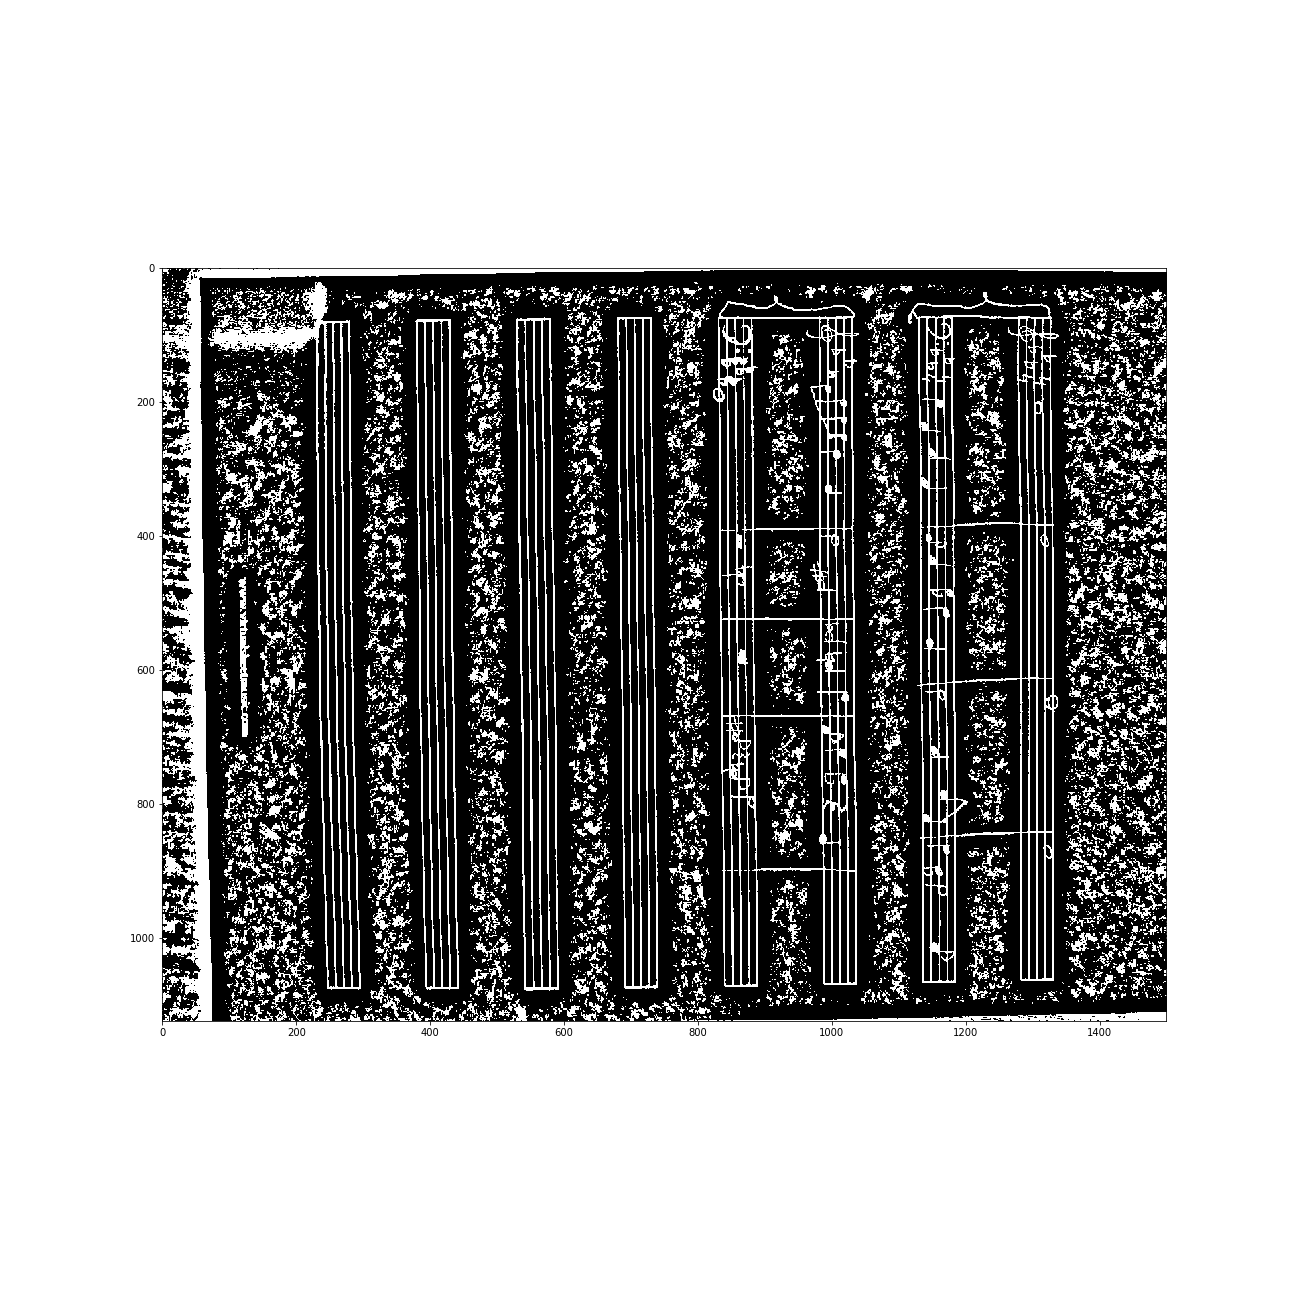
\includegraphics[width=\linewidth]{zdj/Bin0.png}
			\caption{Binaryzacja}
		\end{subfigure}
		\begin{subfigure}[b]{0.32\linewidth}
			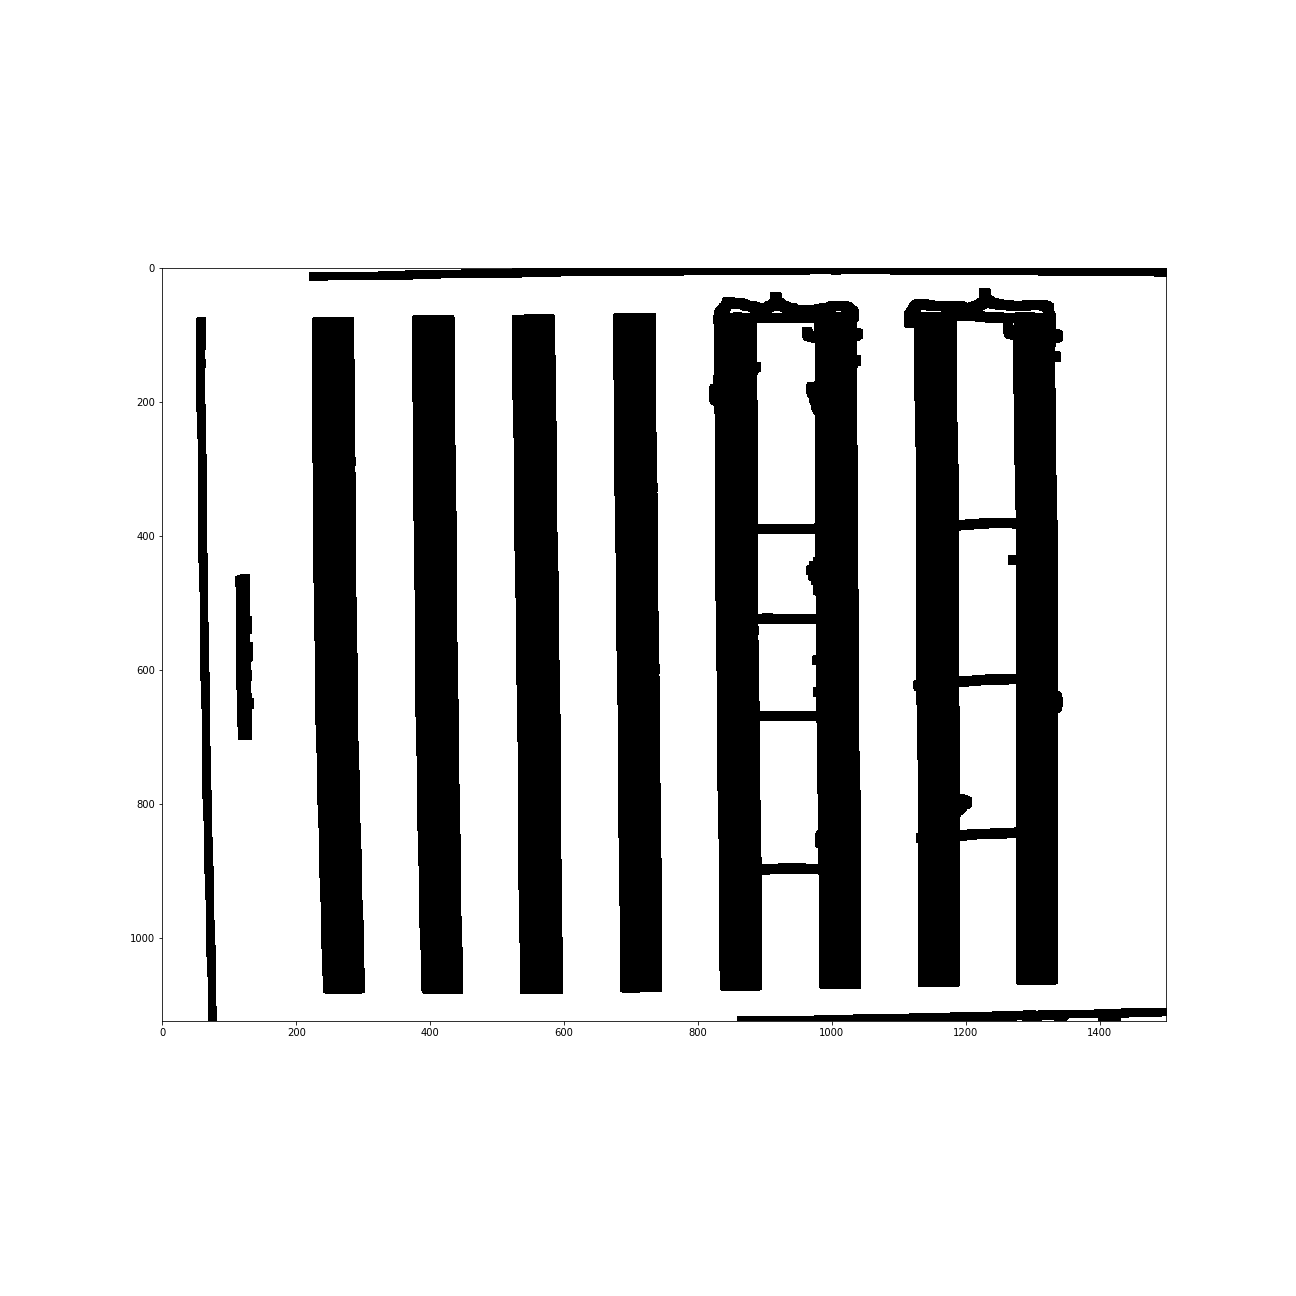
\includegraphics[width=\linewidth]{zdj/Bin1.png}
			\caption{Blob}
		\end{subfigure}
		\begin{subfigure}[b]{0.32\linewidth}
			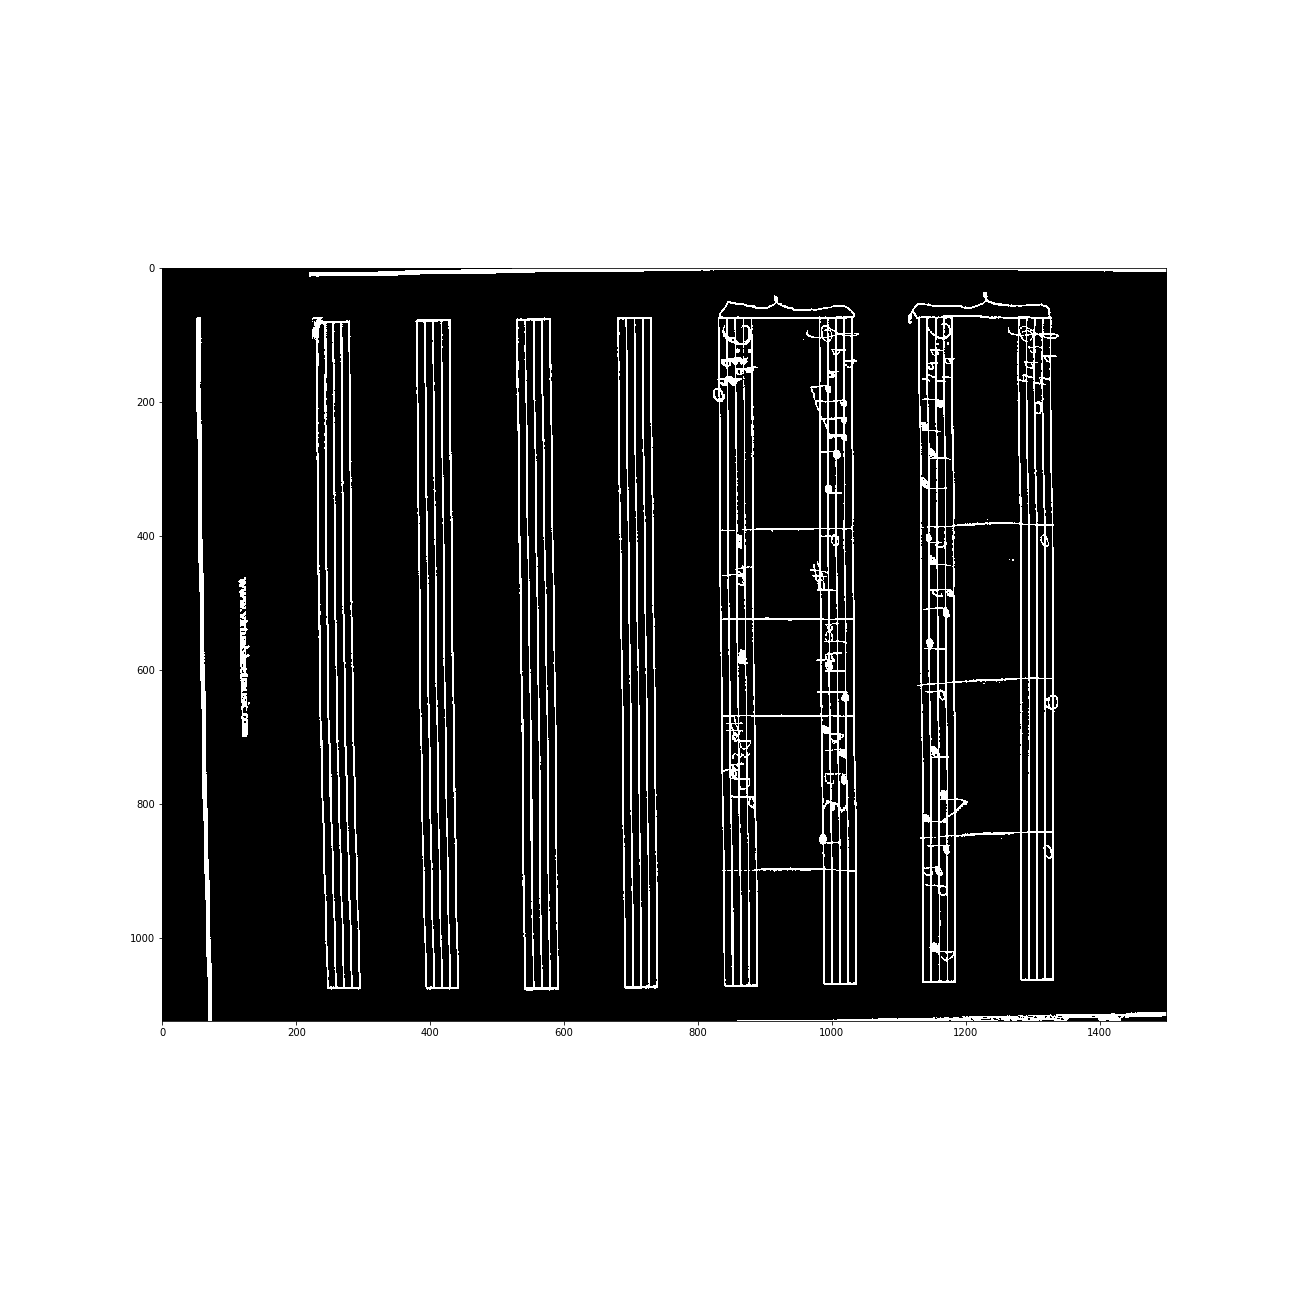
\includegraphics[width=\linewidth]{zdj/Bin2.png}
			\caption{Oczyszczona binaryzacja}
		\end{subfigure}
		\caption{Proces Binaryzacji.}
		\label{fig:binary}
	\end{figure}

	\begin{figure}[h!]
		\centering
		\begin{subfigure}[b]{0.48\linewidth}
			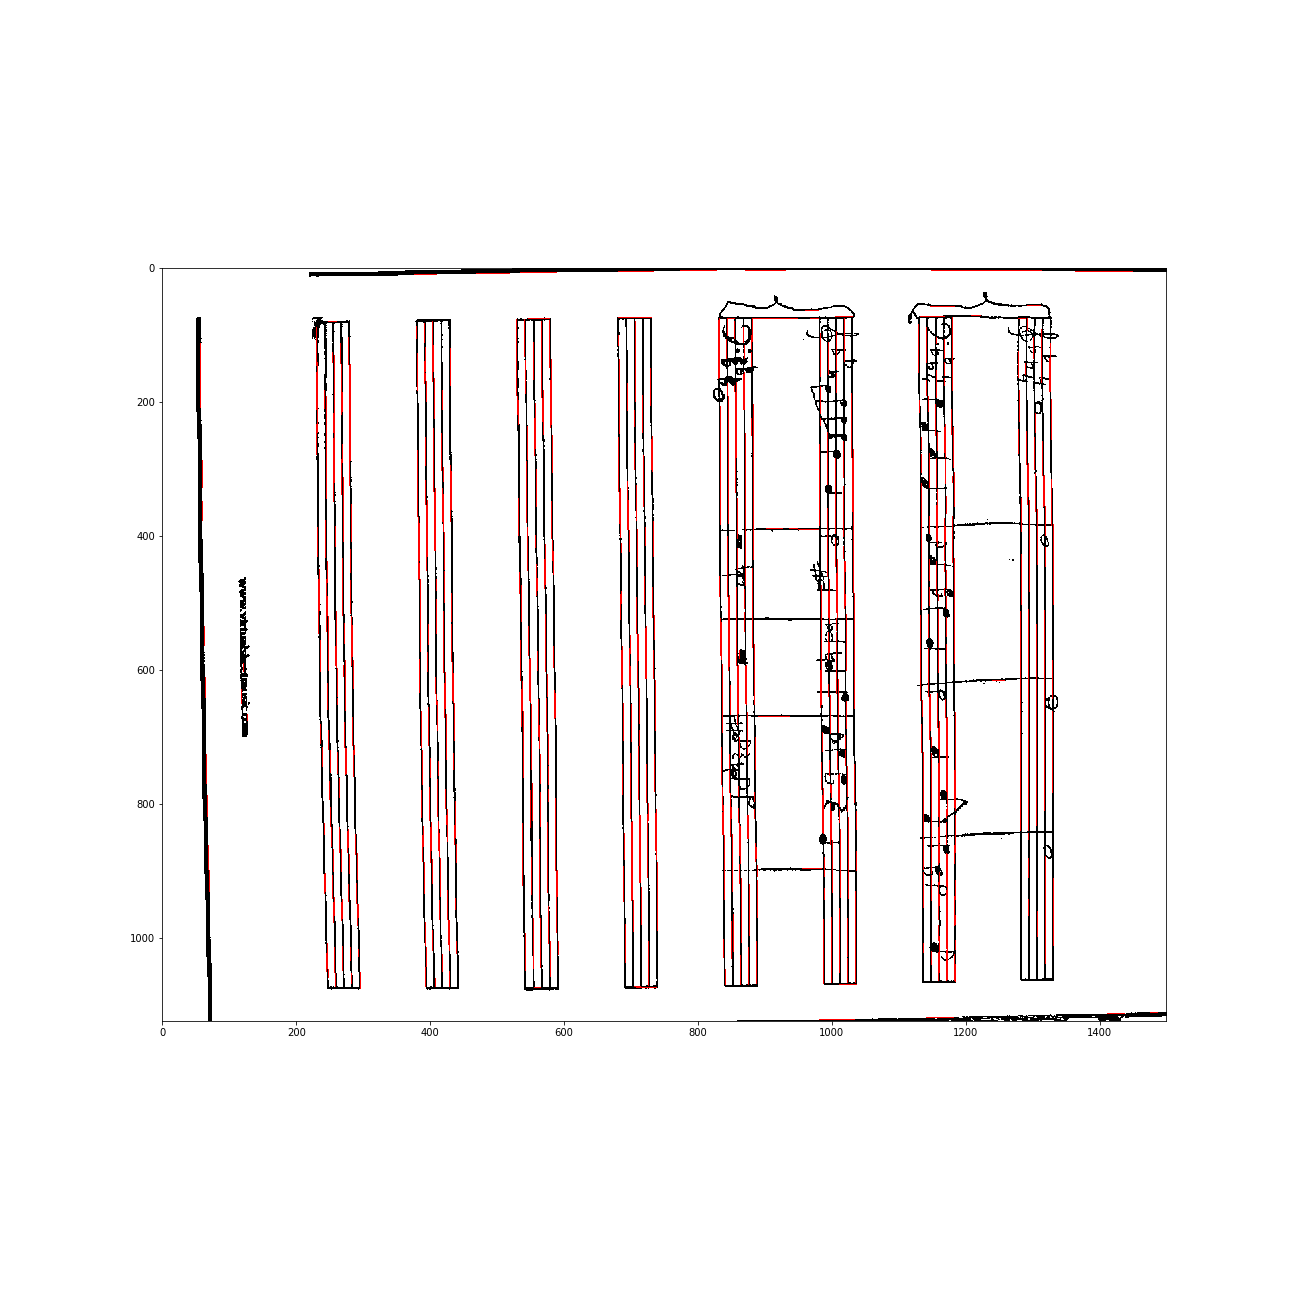
\includegraphics[width=\linewidth]{zdj/Rot0.png}
			\caption{Linie proste}
		\end{subfigure}
		\begin{subfigure}[b]{0.48\linewidth}
			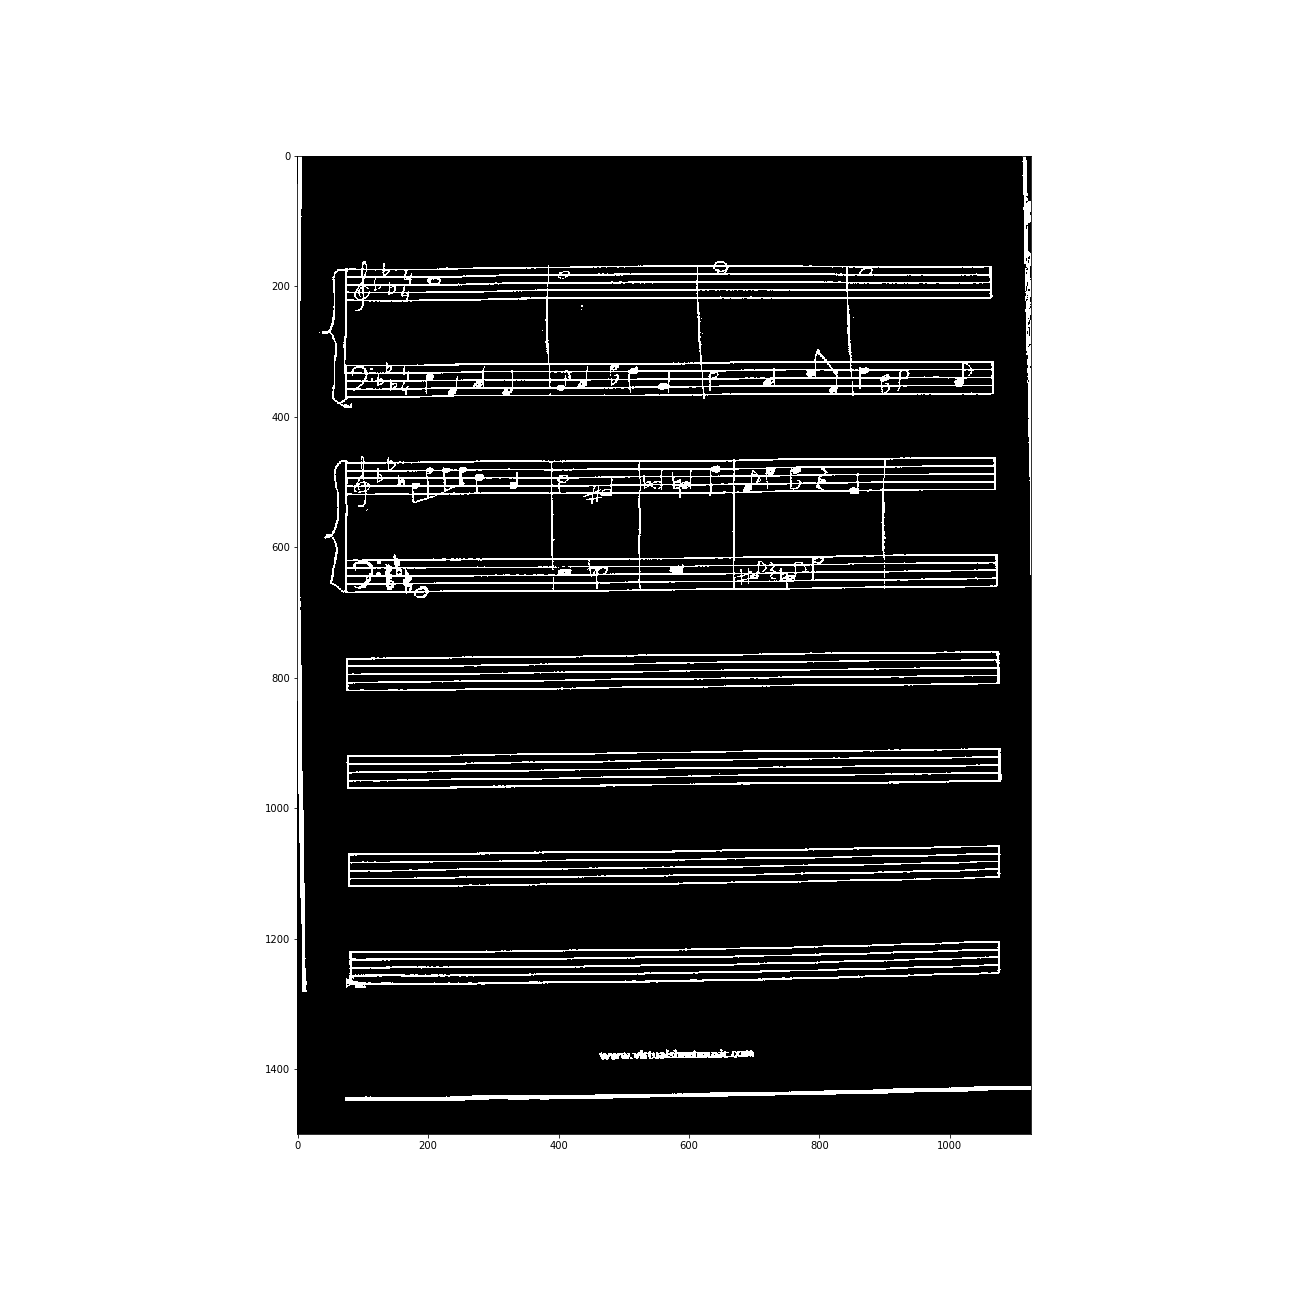
\includegraphics[width=\linewidth]{zdj/Rot1.png}
			\caption{Obrót}
		\end{subfigure}
		\caption{Proces Rotacji.}
		\label{fig:rotate}
	\end{figure}

	\begin{figure}[h!]
		\begin{subfigure}[b]{0.32\linewidth}
			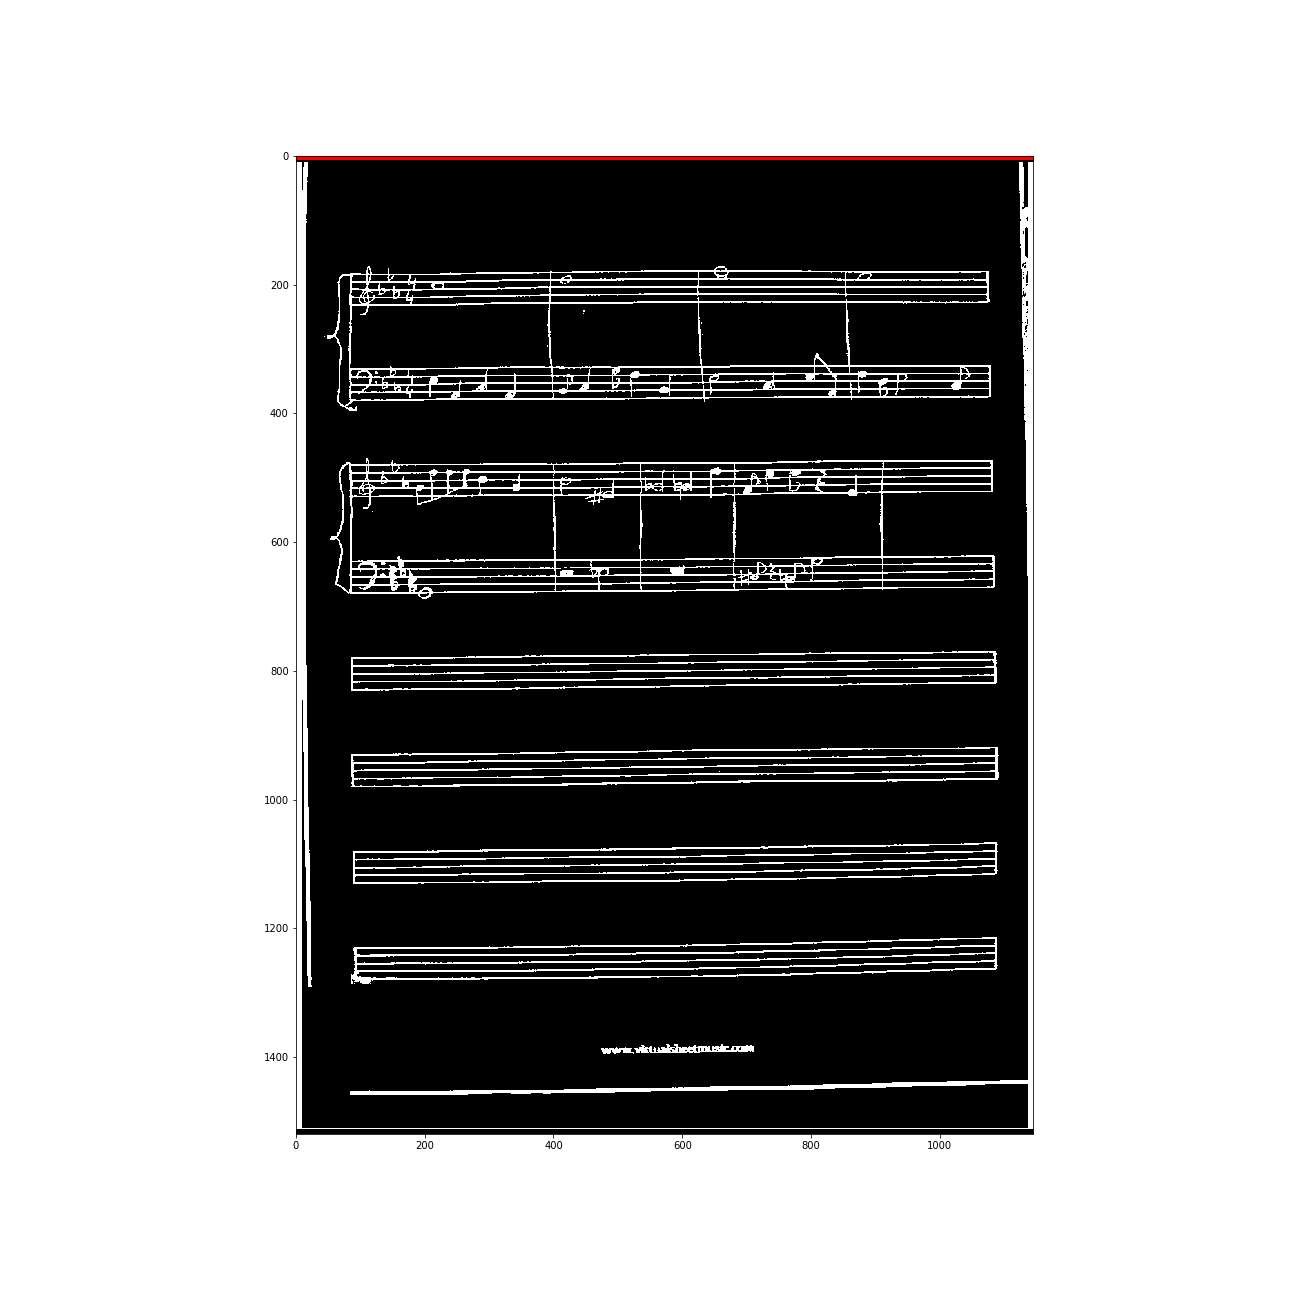
\includegraphics[width=\linewidth]{zdj/BFS0.png}
		\end{subfigure}
		\begin{subfigure}[b]{0.32\linewidth}
			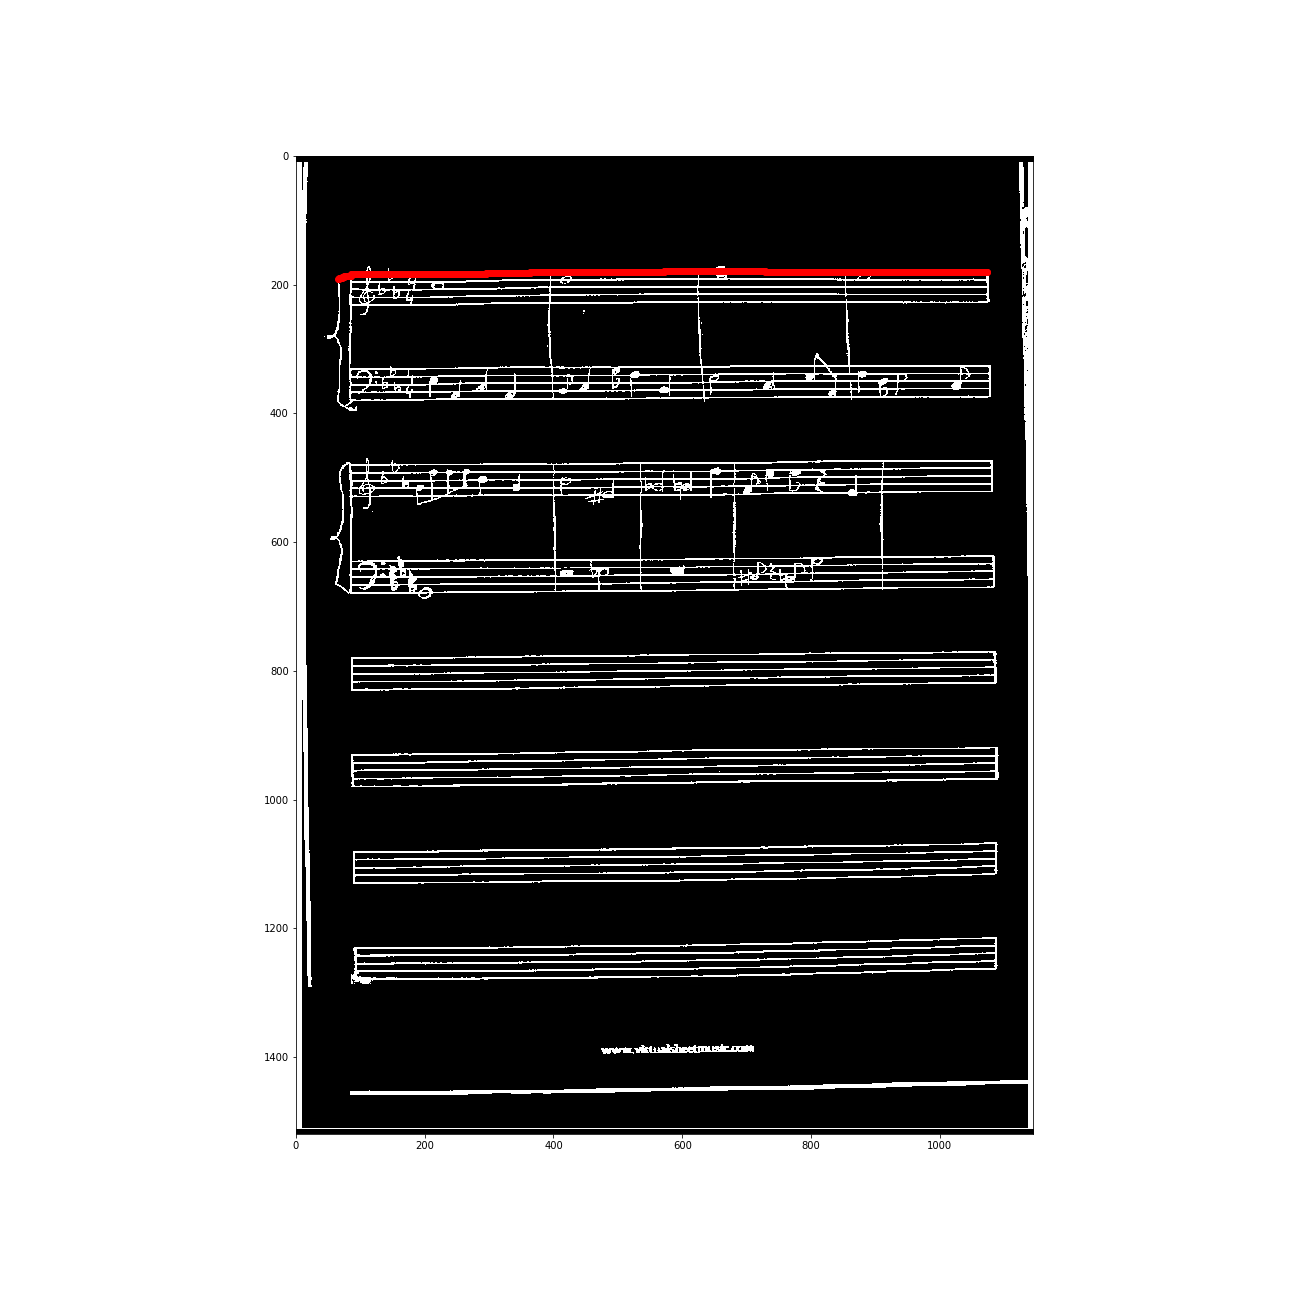
\includegraphics[width=\linewidth]{zdj/BFS1.png}
		\end{subfigure}
		\begin{subfigure}[b]{0.32\linewidth}
			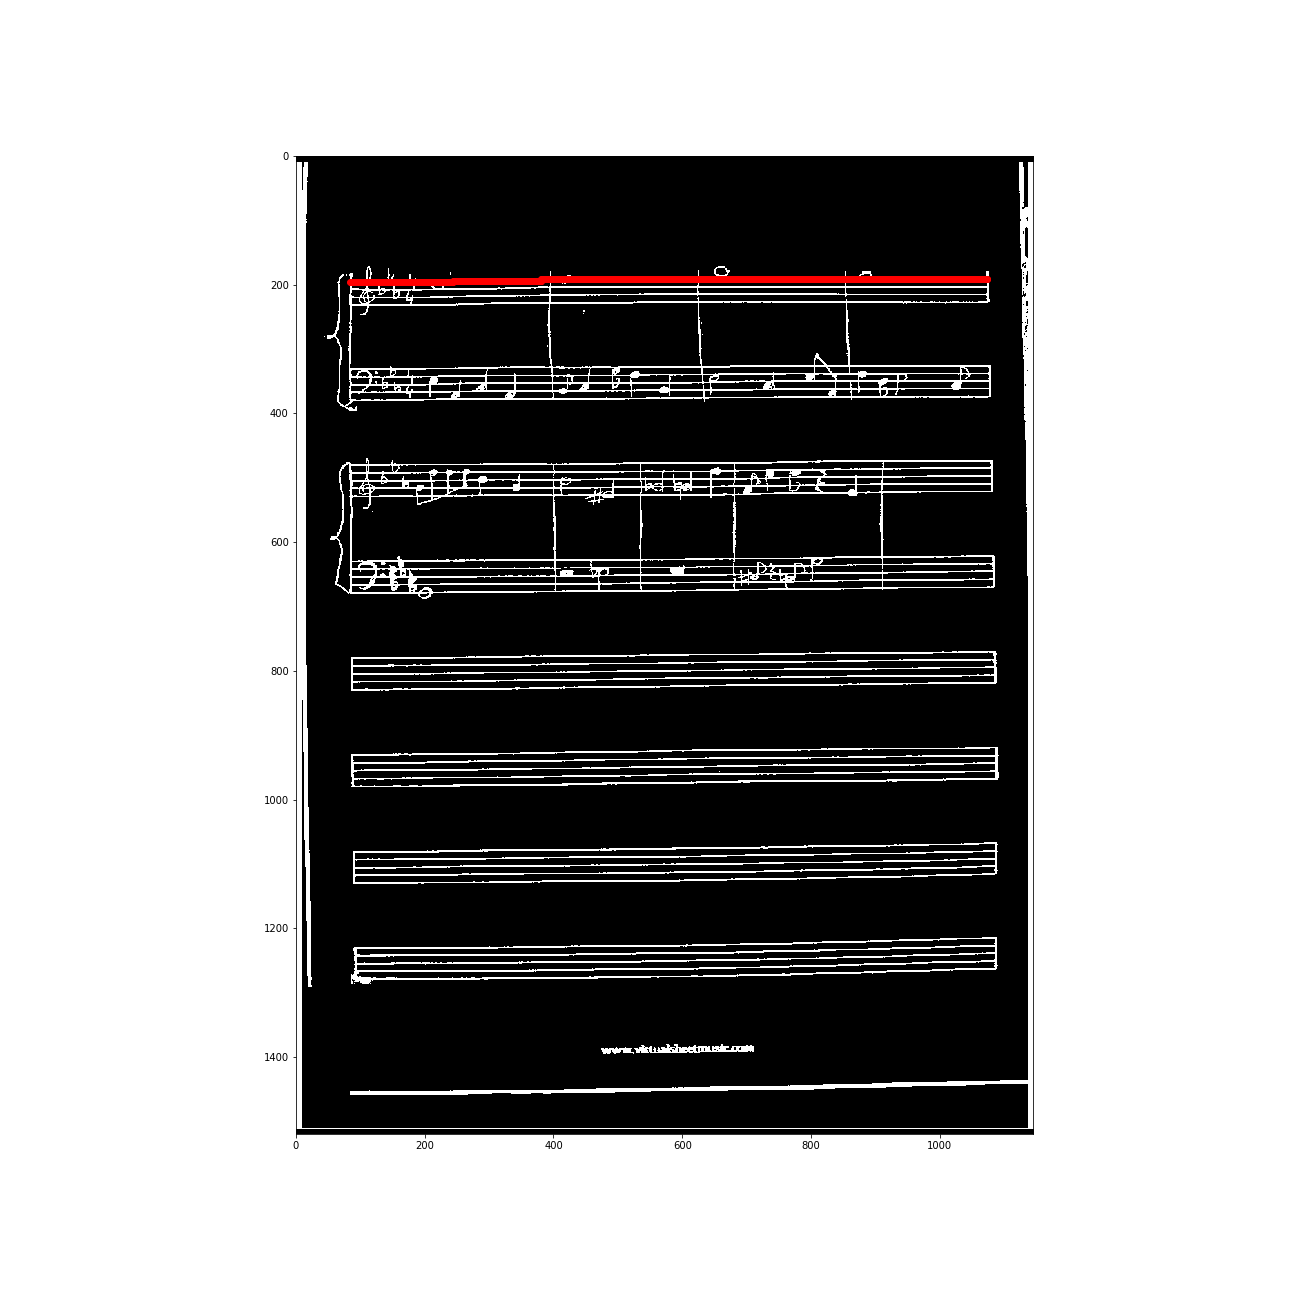
\includegraphics[width=\linewidth]{zdj/BFS2.png}
		\end{subfigure}
		\begin{subfigure}[b]{0.32\linewidth}
			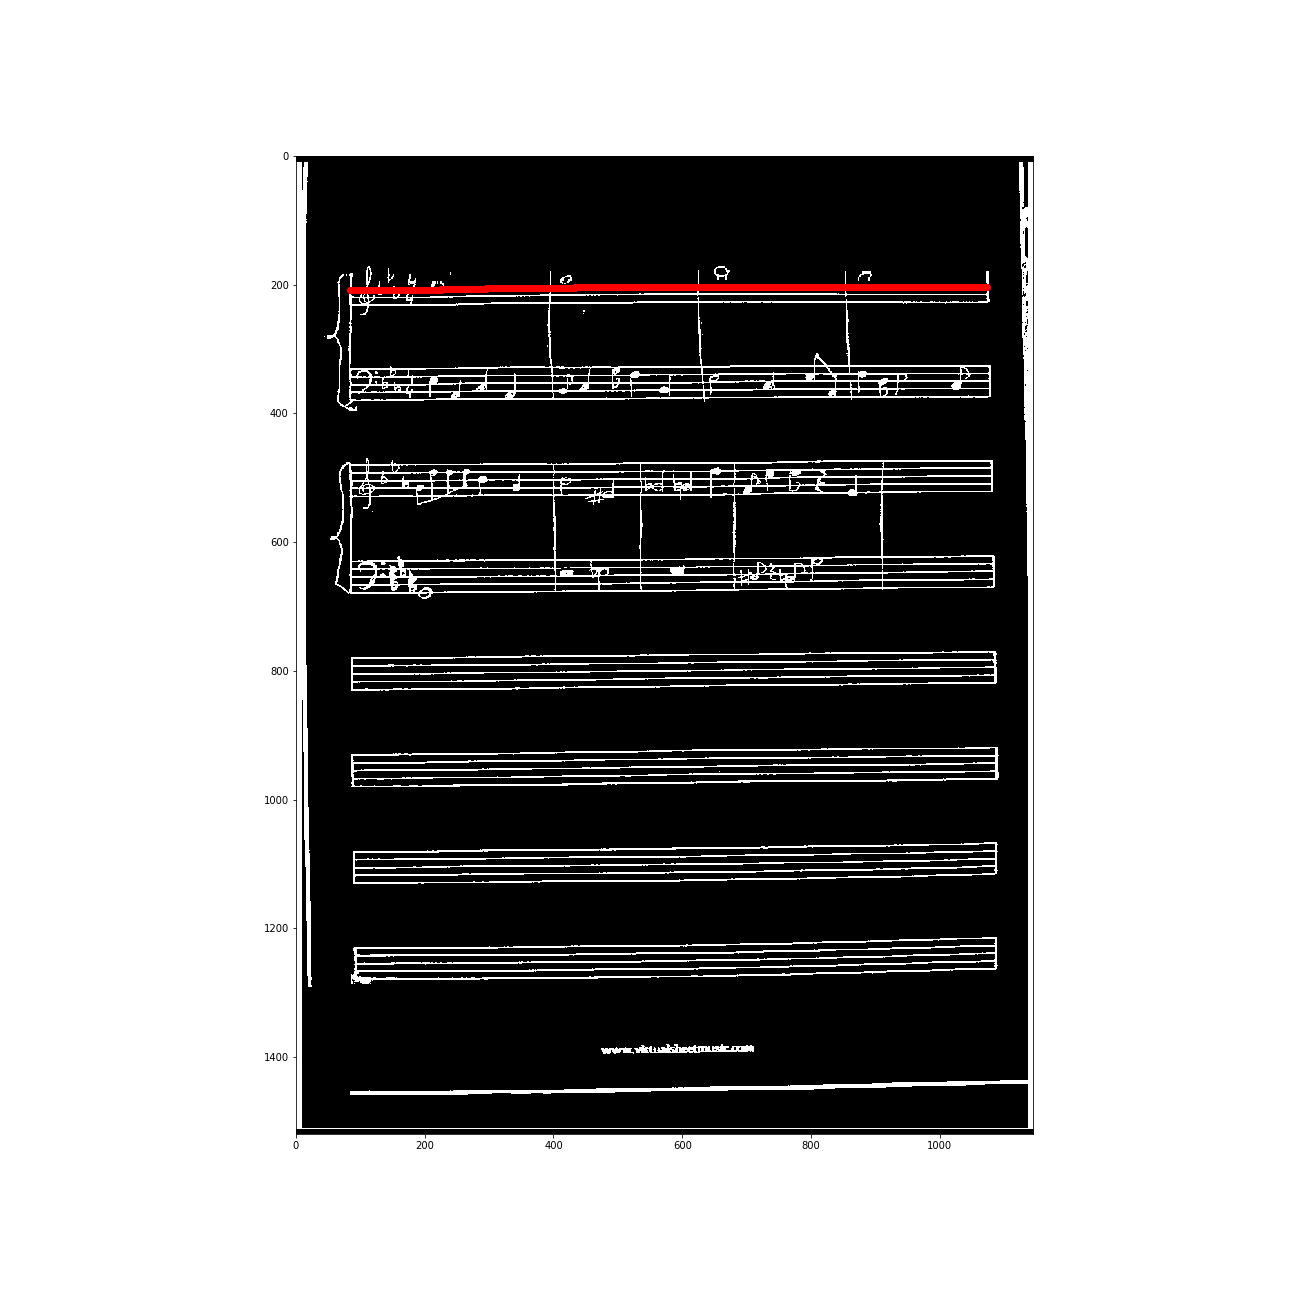
\includegraphics[width=\linewidth]{zdj/BFS3.png}
		\end{subfigure}
		\begin{subfigure}[b]{0.32\linewidth}
			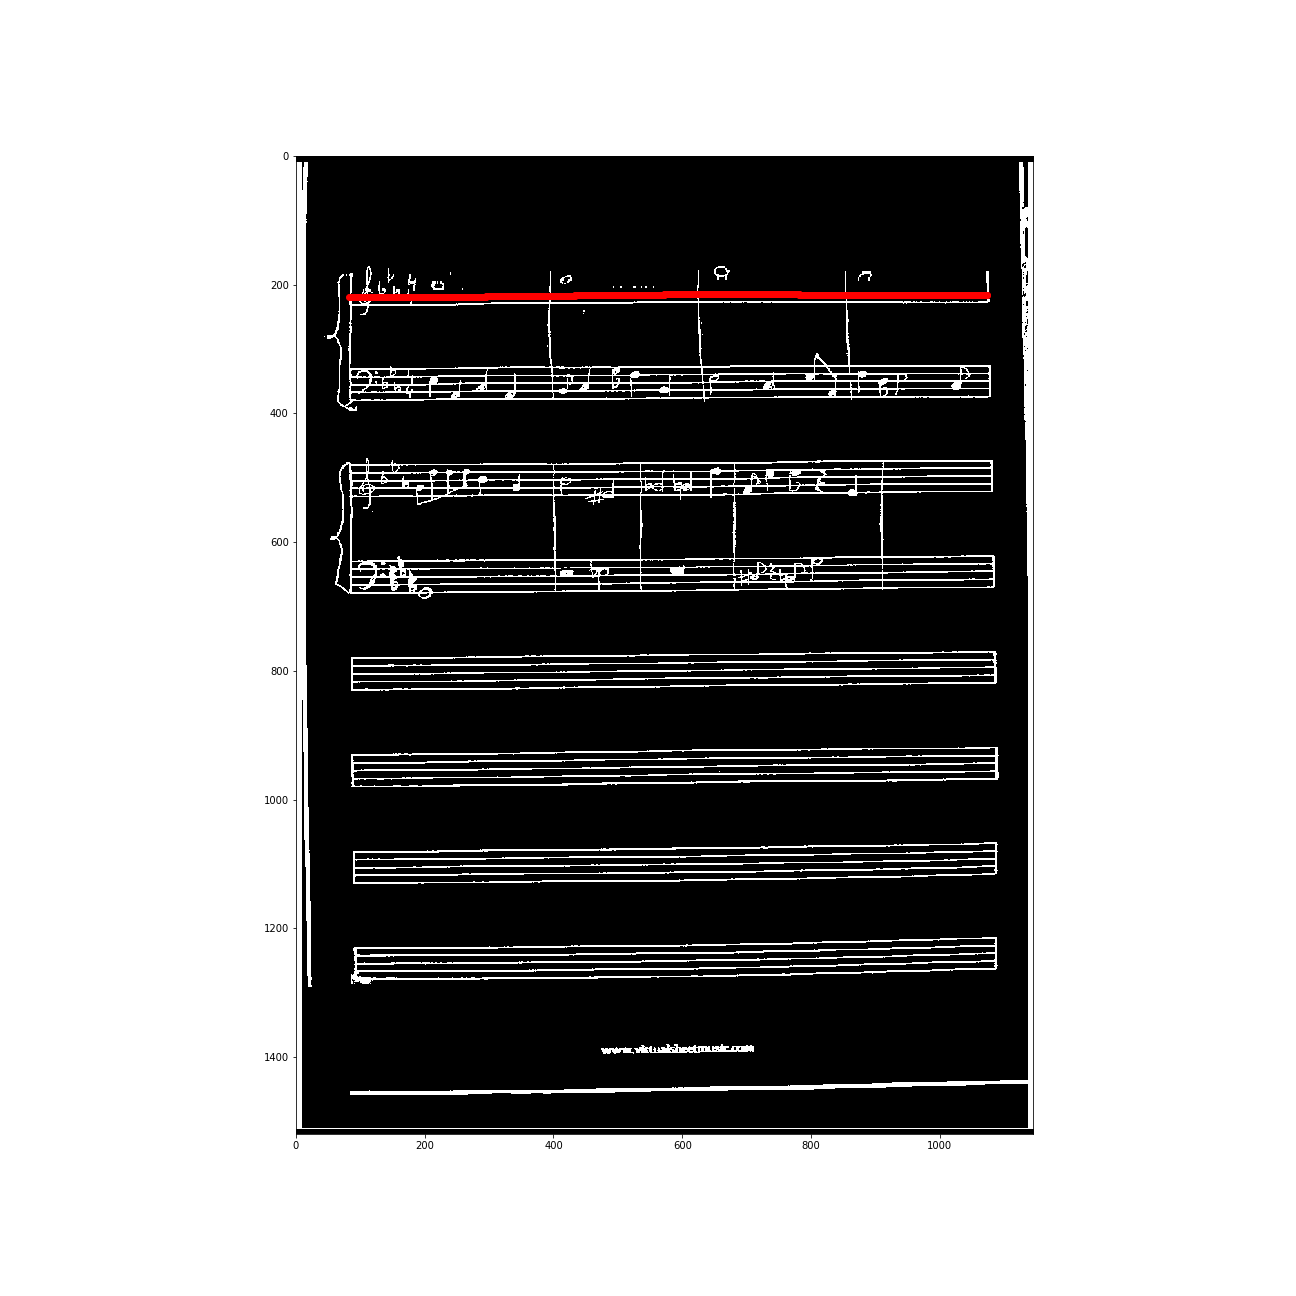
\includegraphics[width=\linewidth]{zdj/BFS4.png}
		\end{subfigure}
		\begin{subfigure}[b]{0.32\linewidth}
			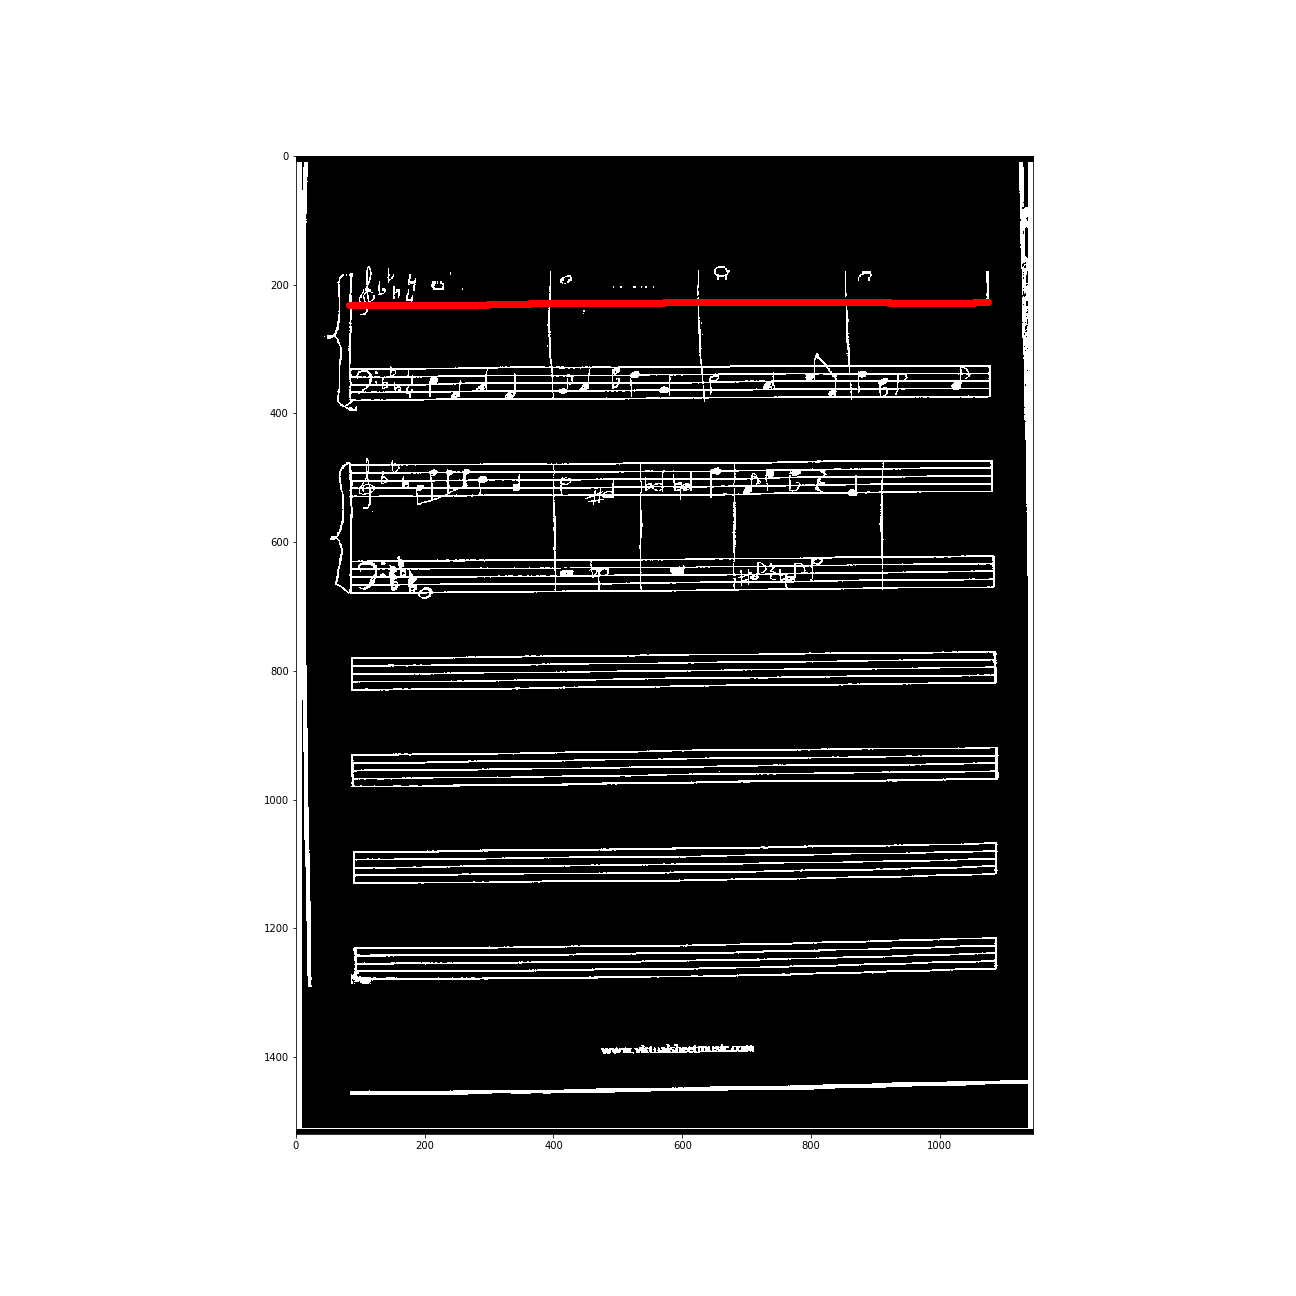
\includegraphics[width=\linewidth]{zdj/BFS5.png}
		\end{subfigure}
		\begin{subfigure}[b]{0.32\linewidth}
			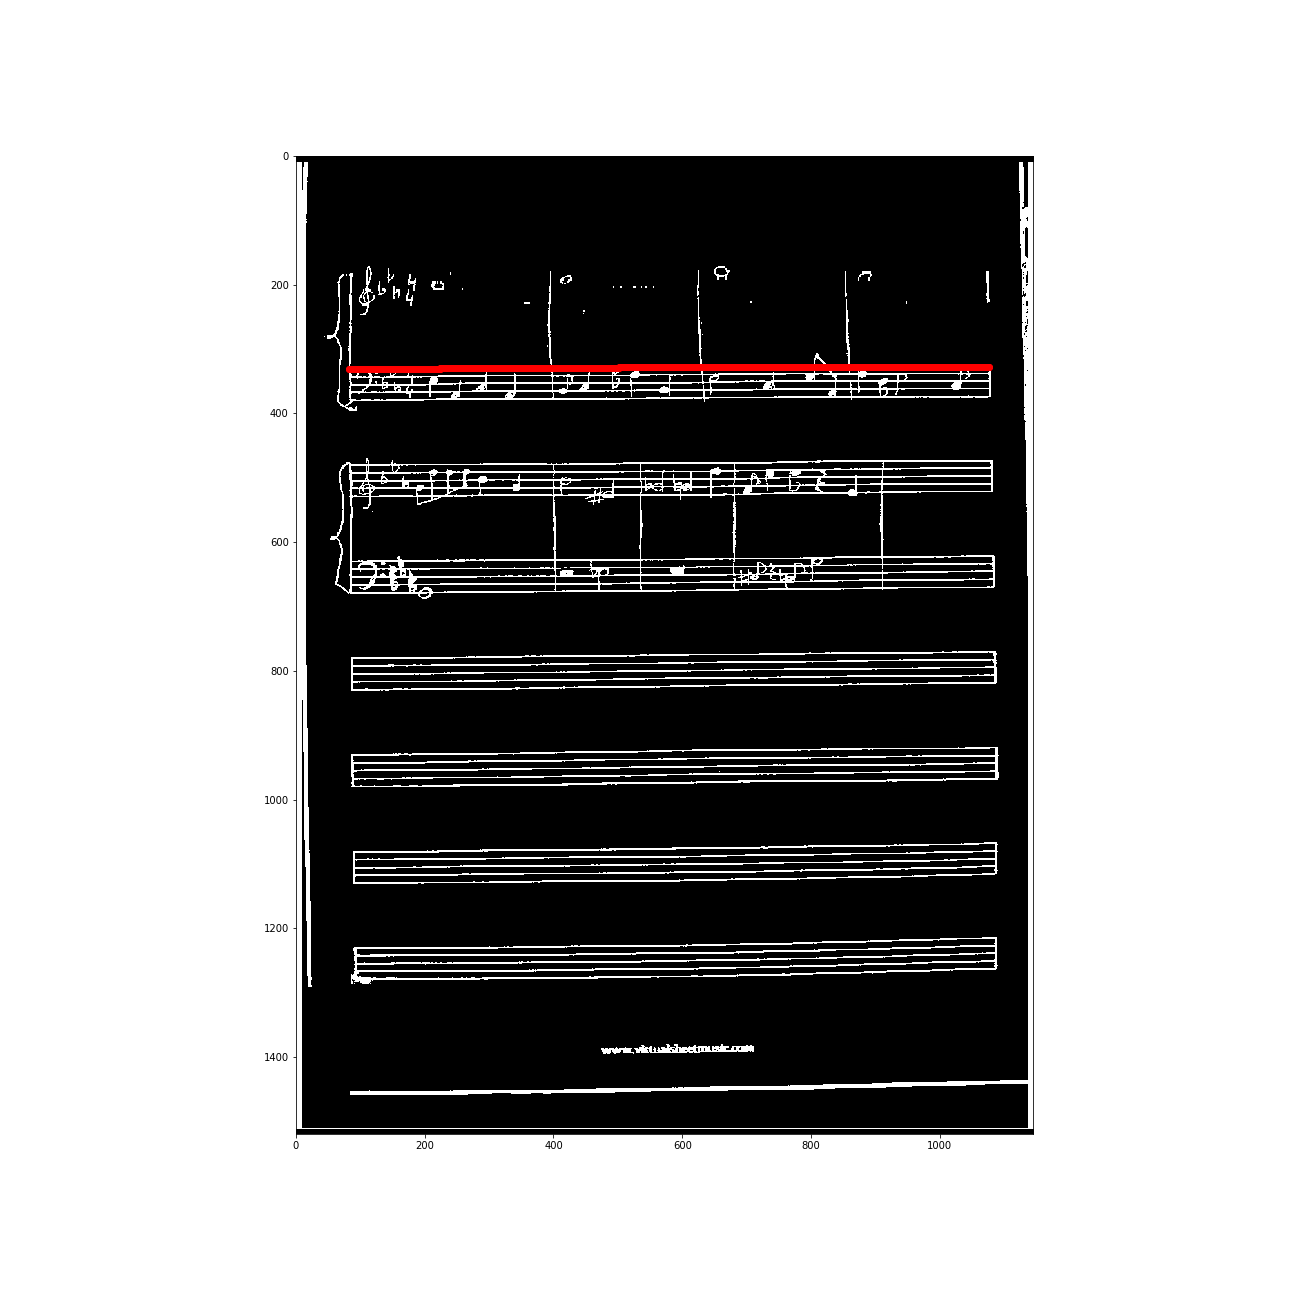
\includegraphics[width=\linewidth]{zdj/BFS6.png}
		\end{subfigure}
		\begin{subfigure}[b]{0.32\linewidth}
			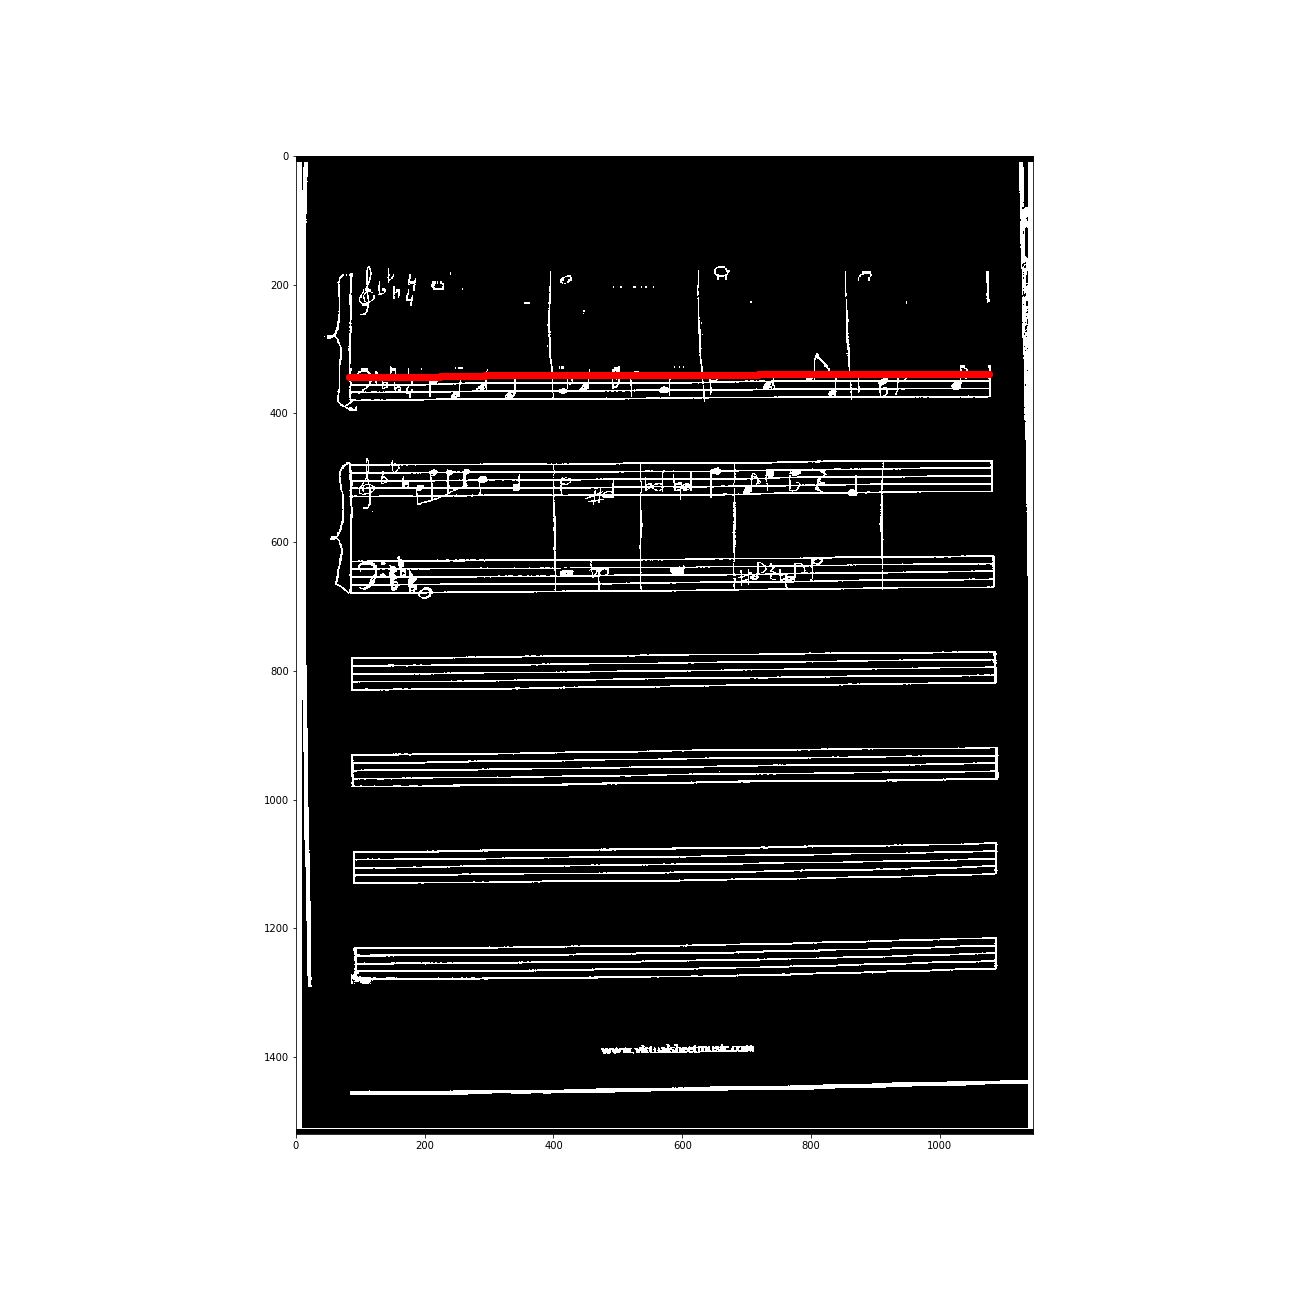
\includegraphics[width=\linewidth]{zdj/BFS7.png}
		\end{subfigure}
		\begin{subfigure}[b]{0.32\linewidth}
			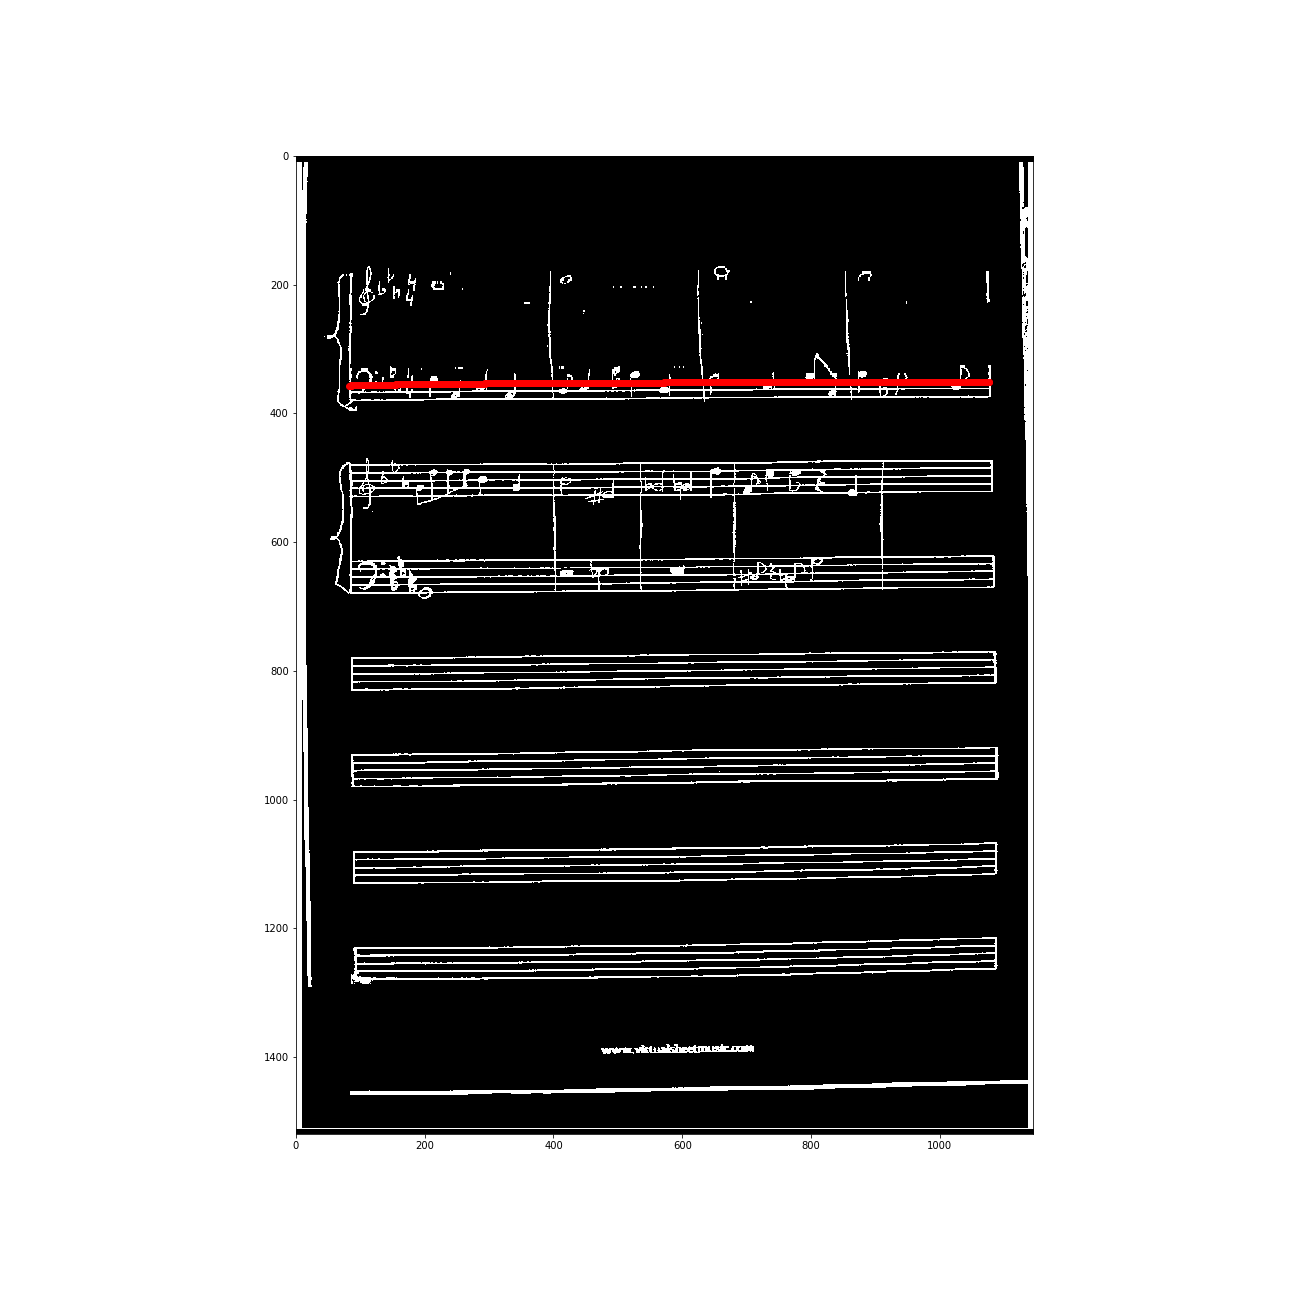
\includegraphics[width=\linewidth]{zdj/BFS8.png}
		\end{subfigure}
		\begin{subfigure}[b]{0.32\linewidth}
			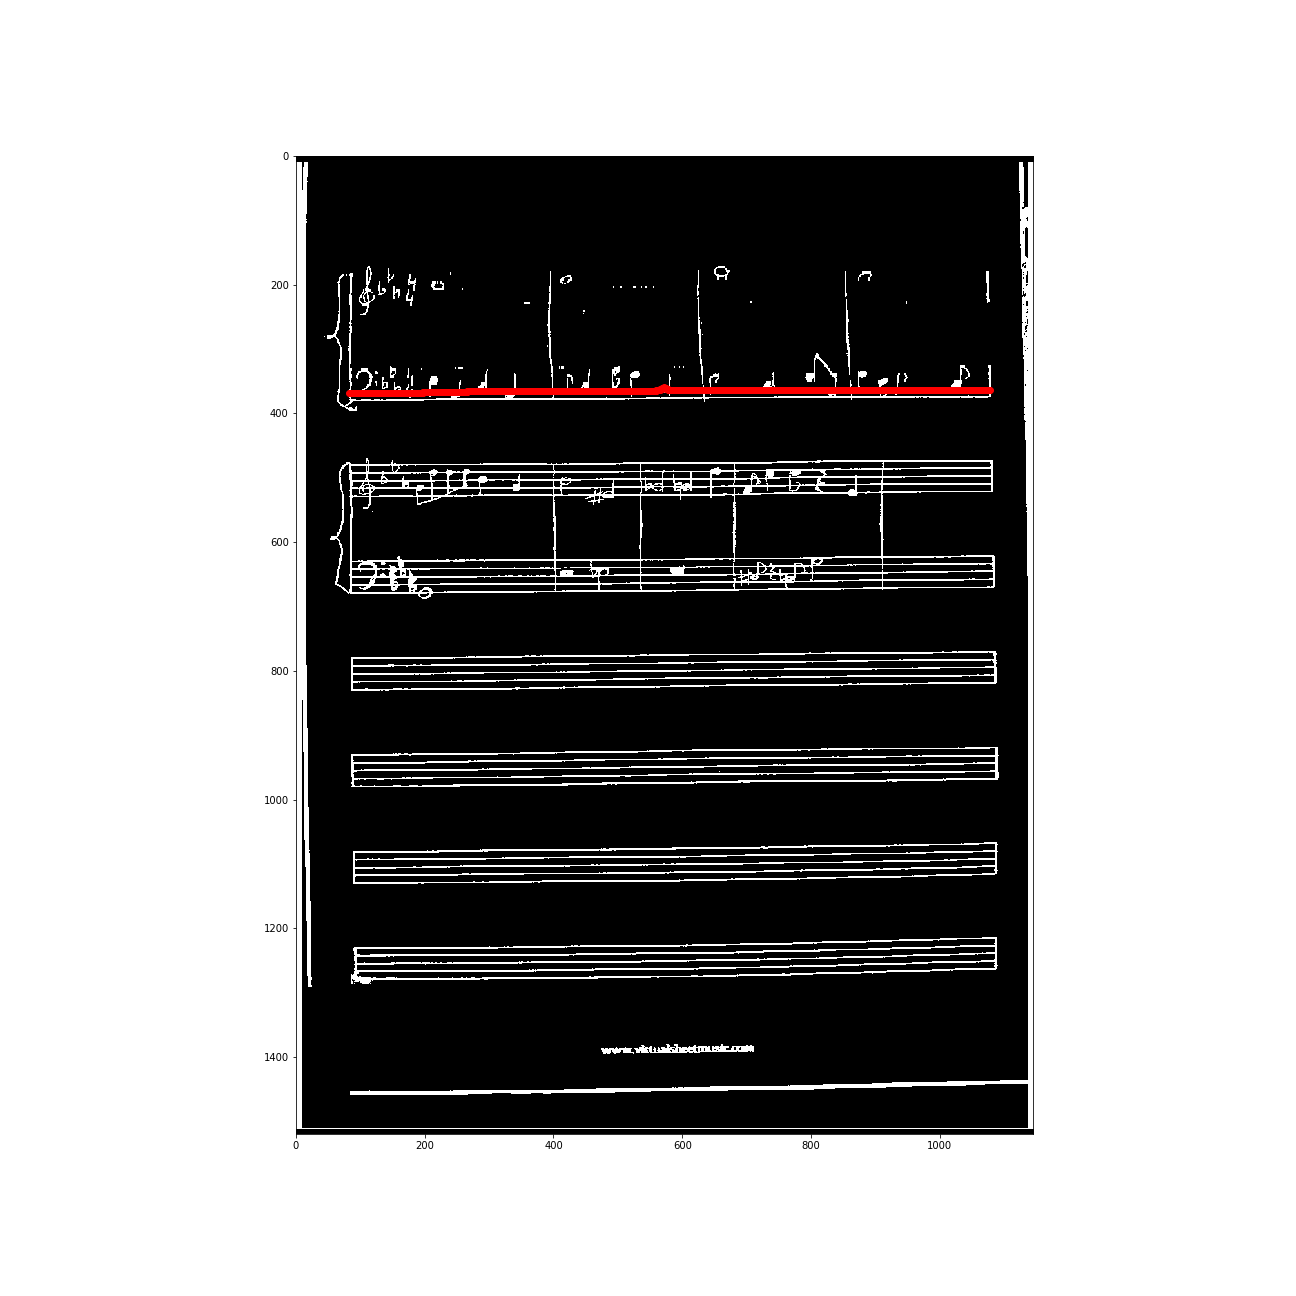
\includegraphics[width=\linewidth]{zdj/BFS9.png}
		\end{subfigure}
		\begin{subfigure}[b]{0.32\linewidth}
			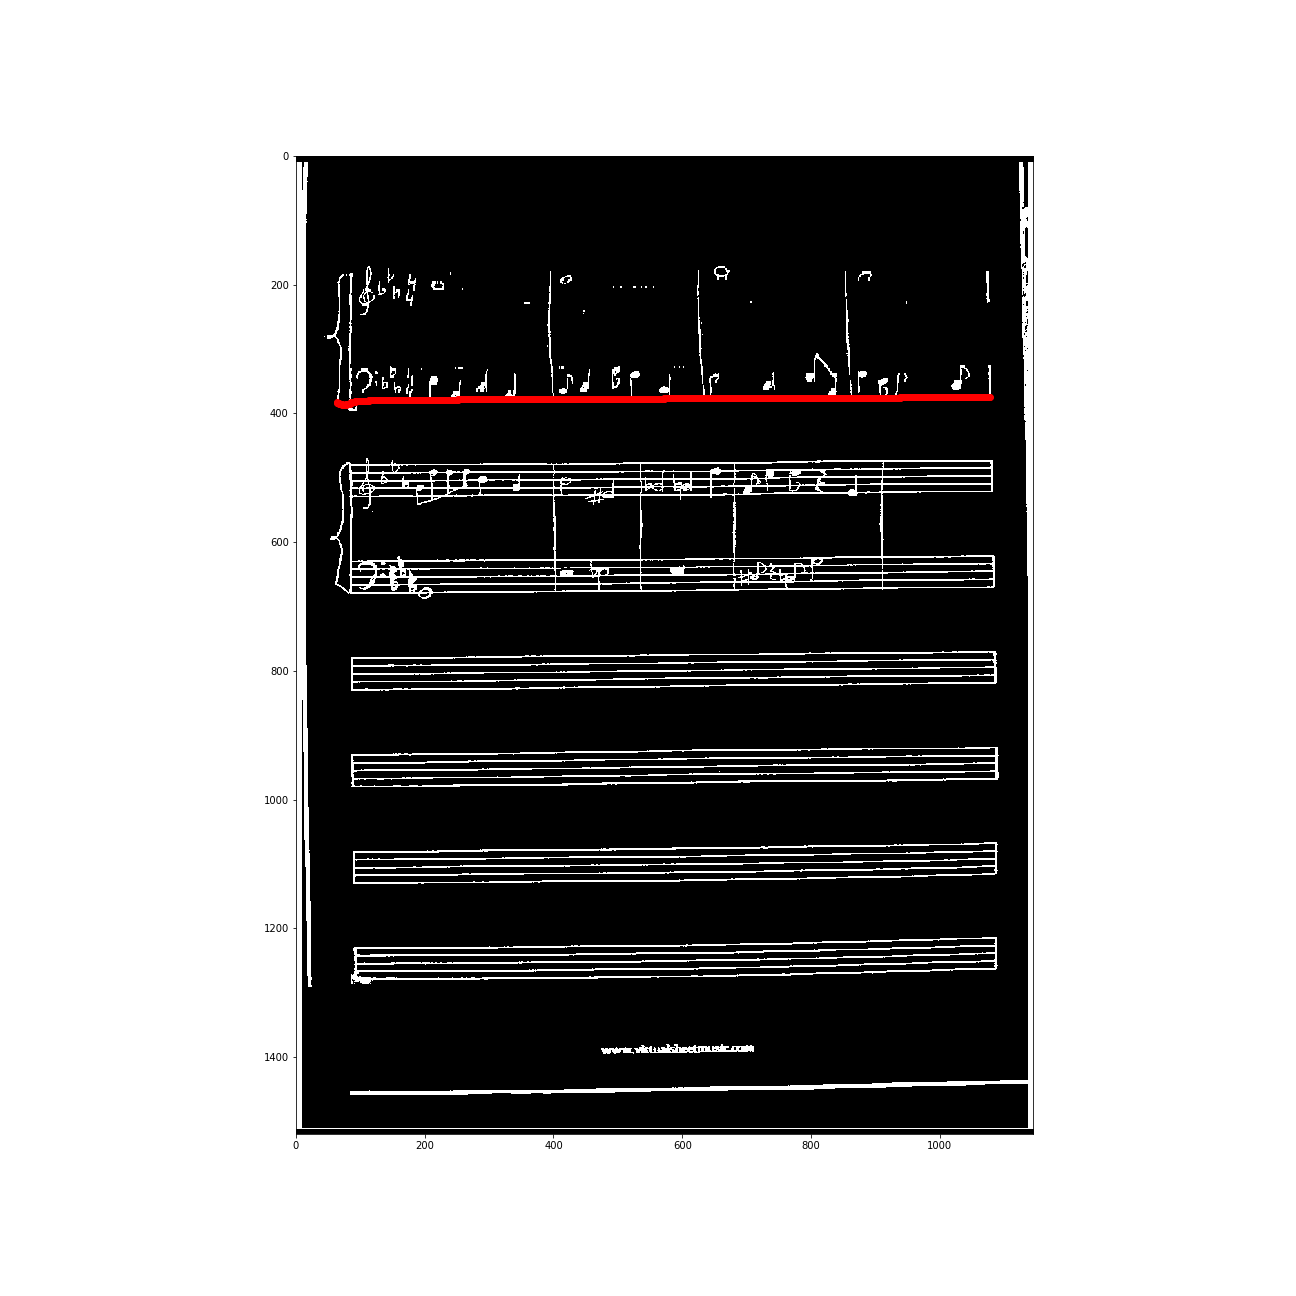
\includegraphics[width=\linewidth]{zdj/BFS10.png}
		\end{subfigure}
		\begin{subfigure}[b]{0.32\linewidth}
			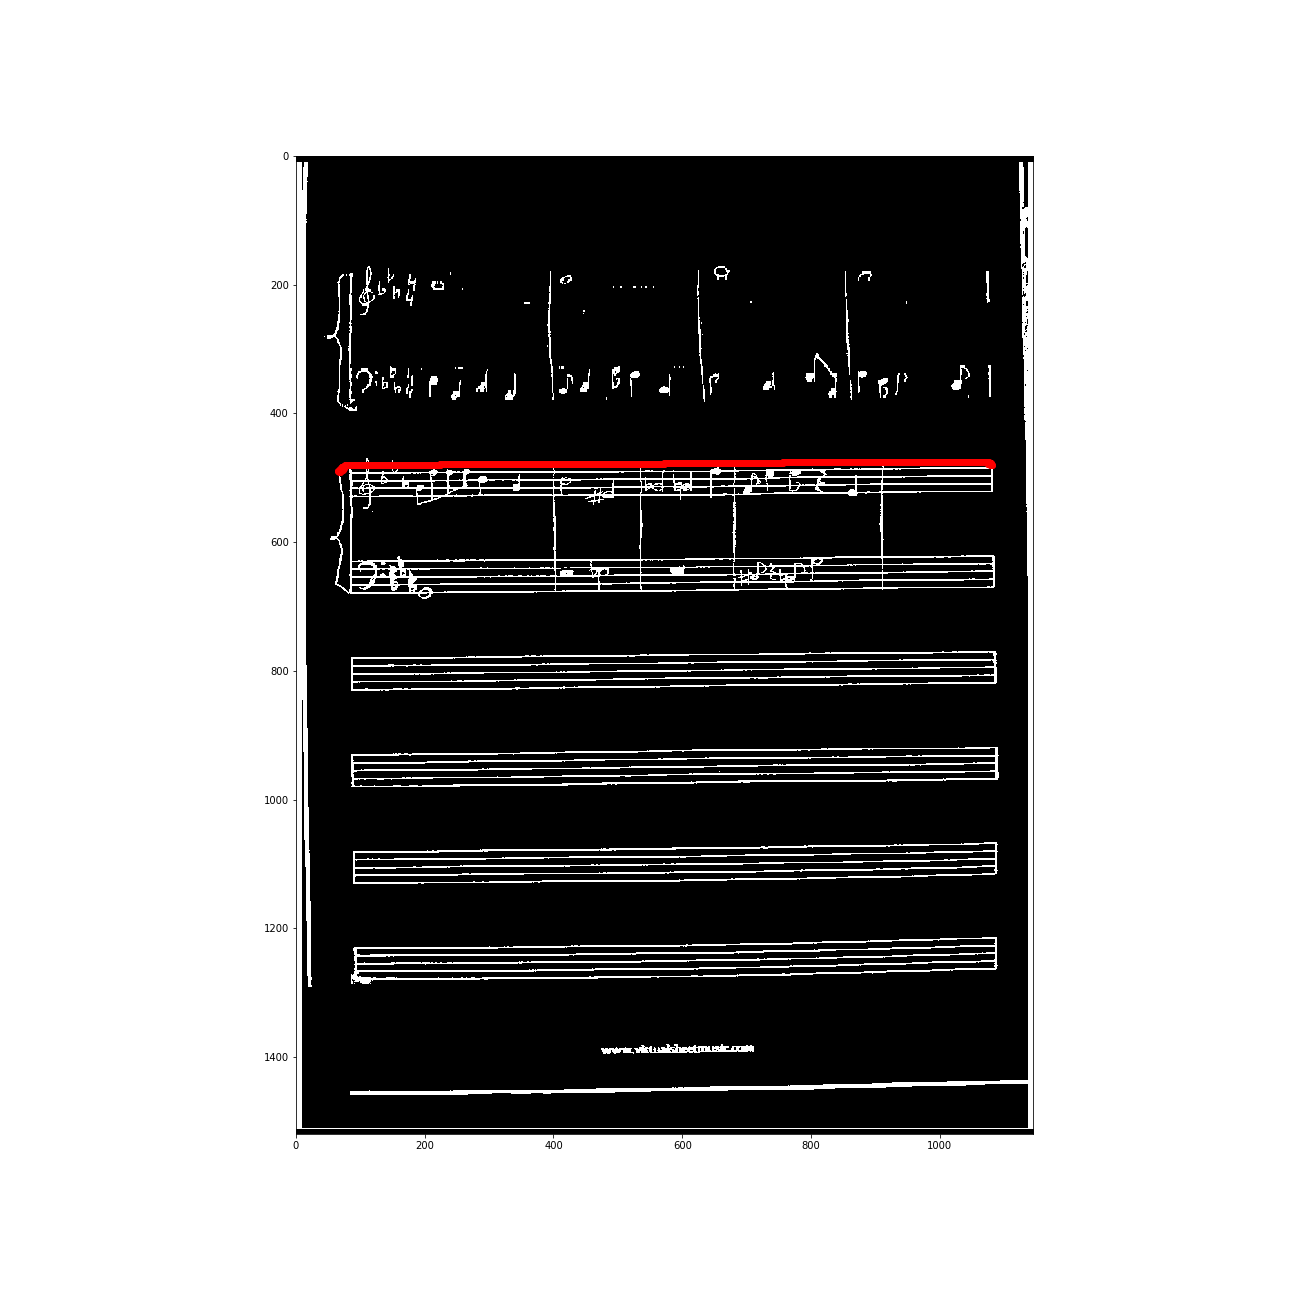
\includegraphics[width=\linewidth]{zdj/BFS11.png}
		\end{subfigure}
		\caption{Proces Detekcji i usuwania linii 1.}
		\label{fig:bfs1}
	\end{figure}

	\begin{figure}[h!]
		\begin{subfigure}[b]{0.32\linewidth}
			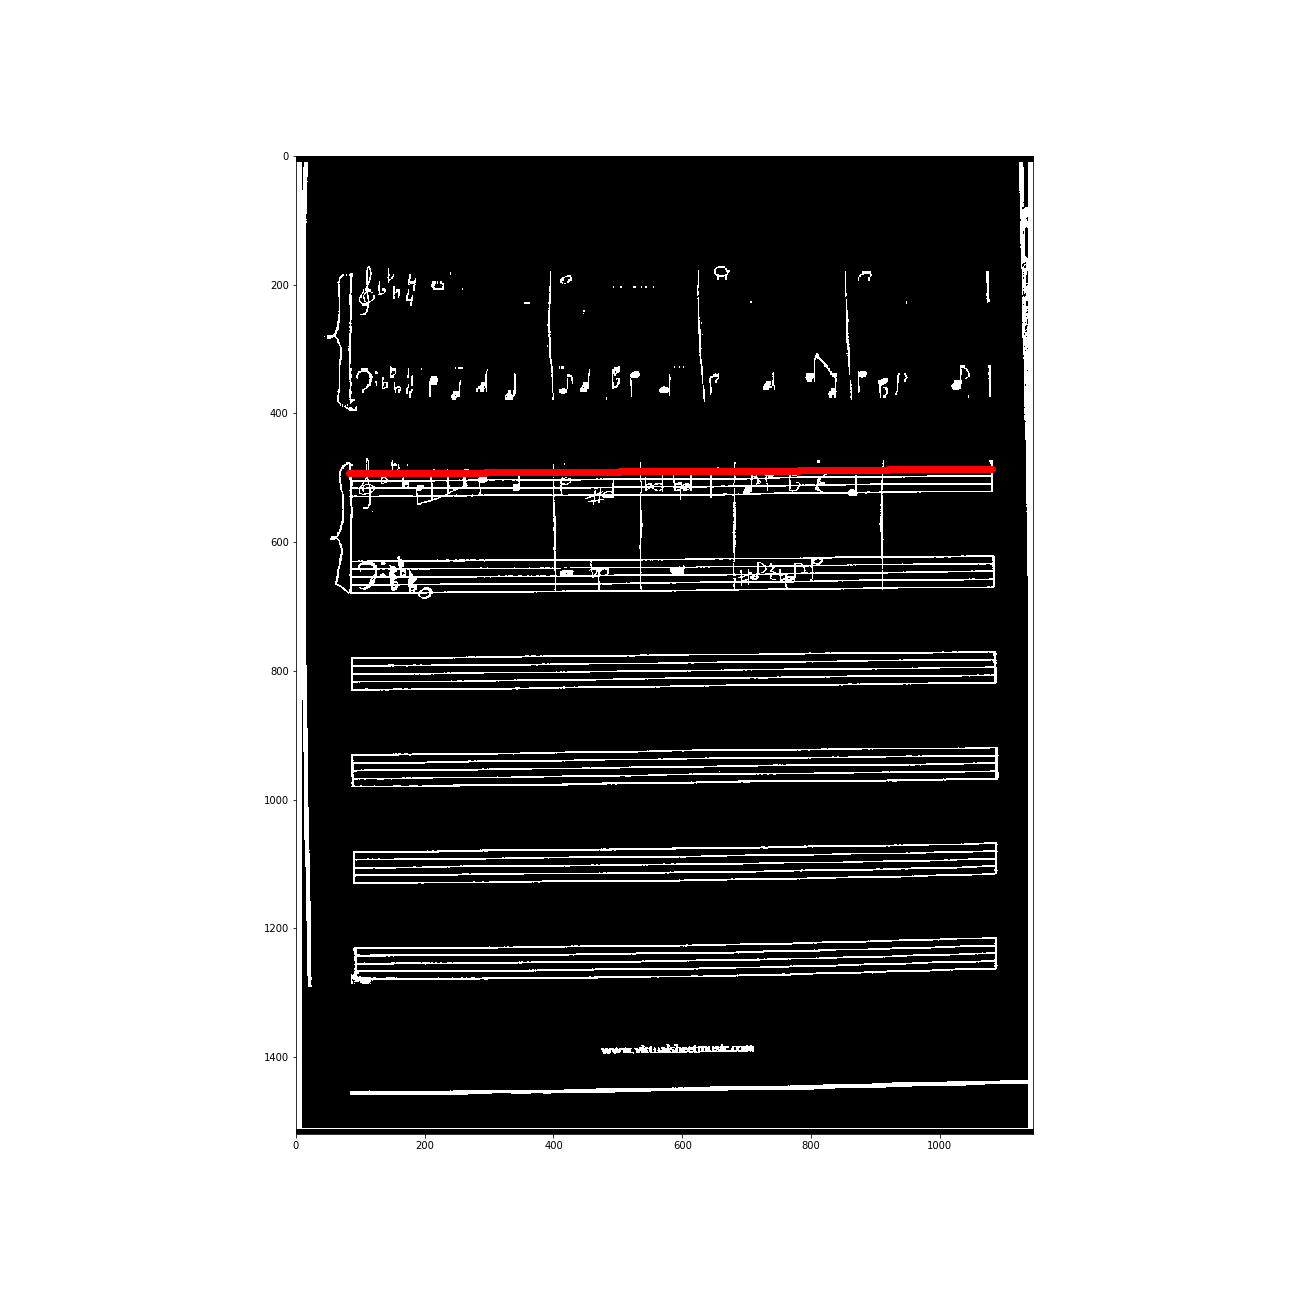
\includegraphics[width=\linewidth]{zdj/BFS12.png}
		\end{subfigure}
		\begin{subfigure}[b]{0.32\linewidth}
			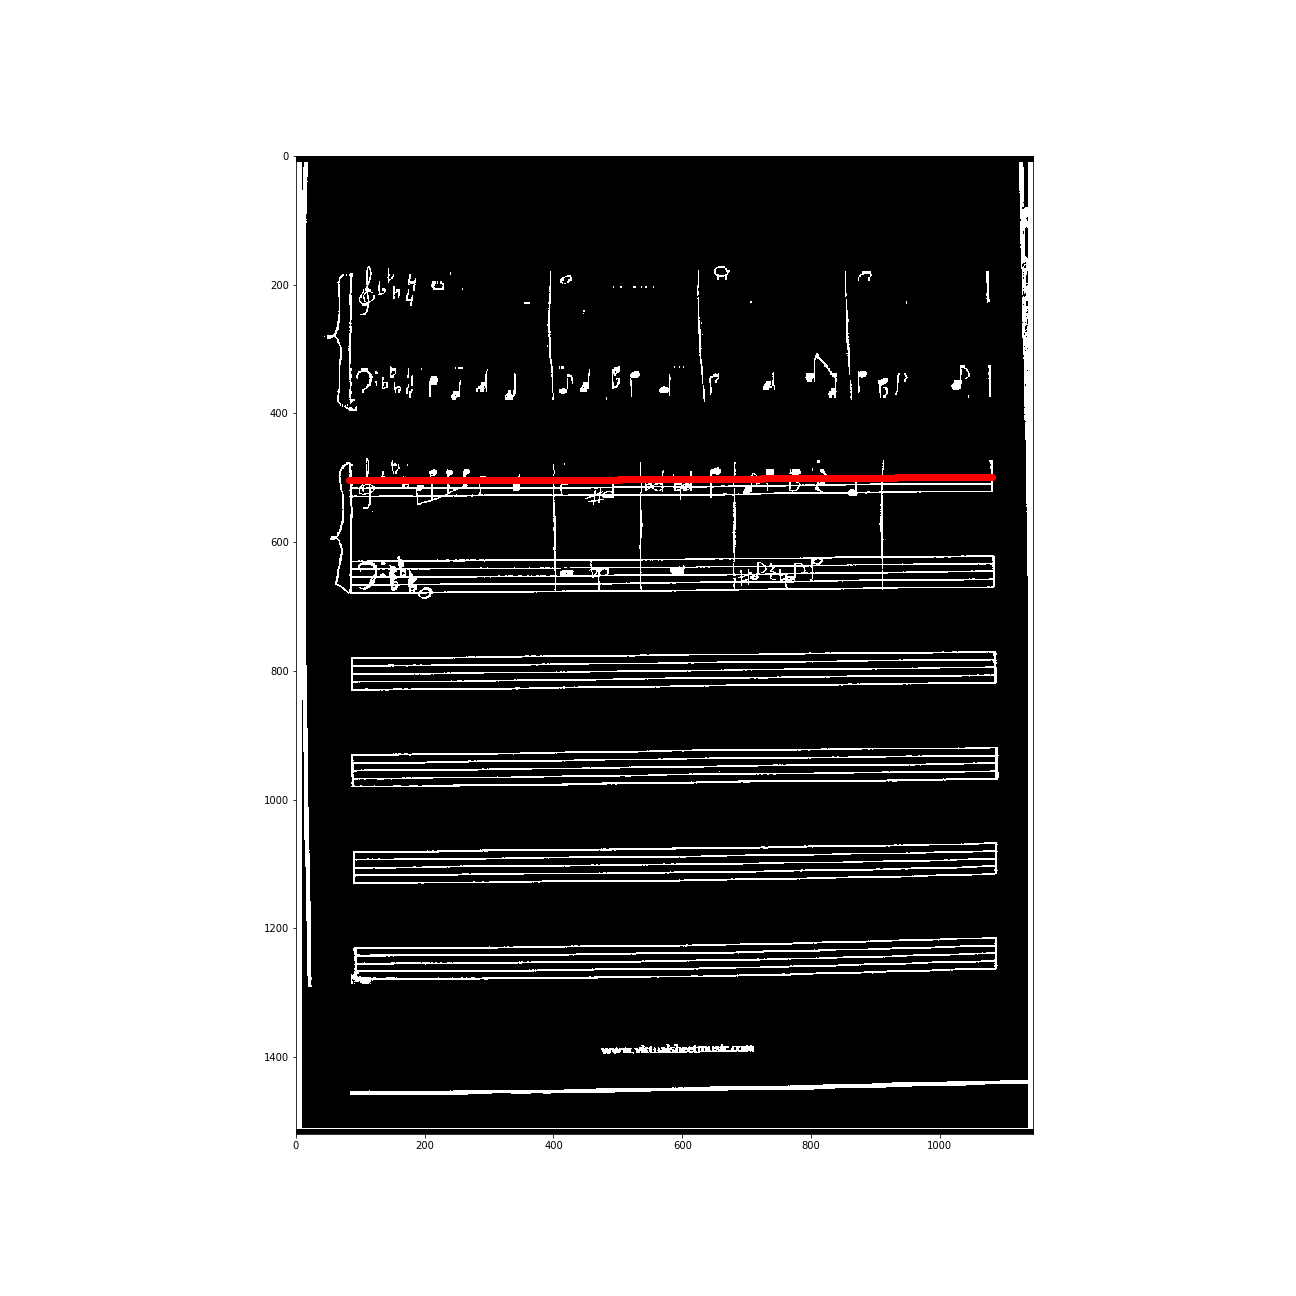
\includegraphics[width=\linewidth]{zdj/BFS13.png}
		\end{subfigure}
		\begin{subfigure}[b]{0.32\linewidth}
			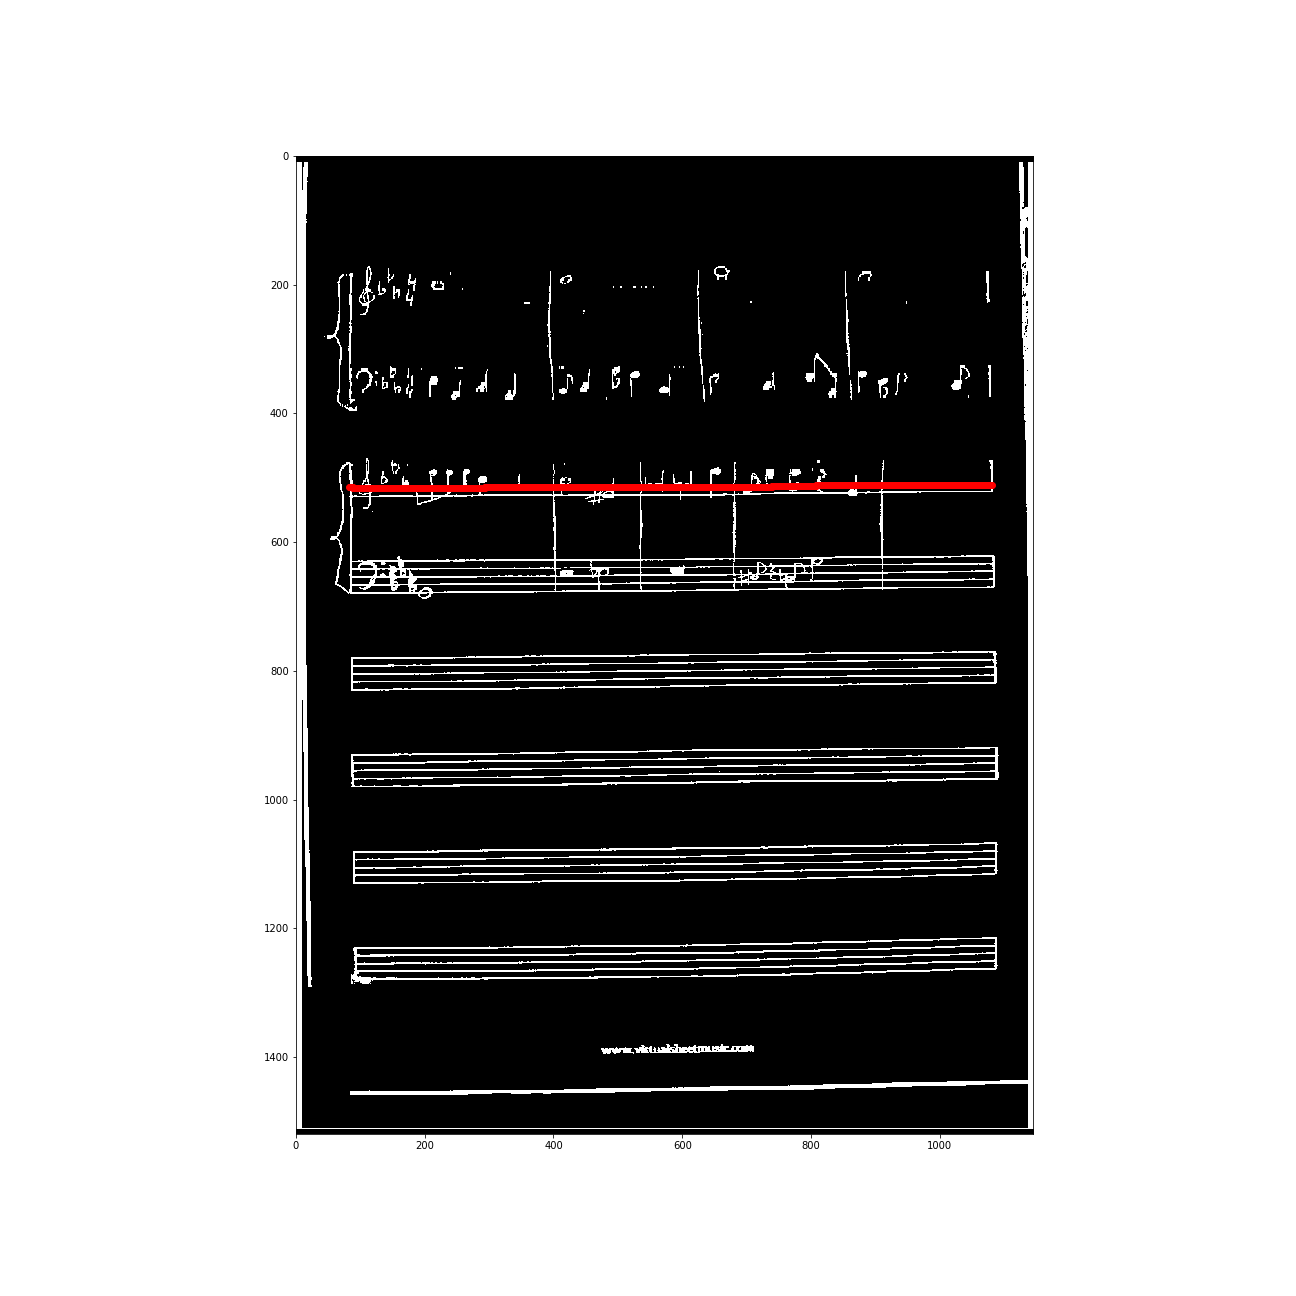
\includegraphics[width=\linewidth]{zdj/BFS14.png}
		\end{subfigure}
		\begin{subfigure}[b]{0.32\linewidth}
			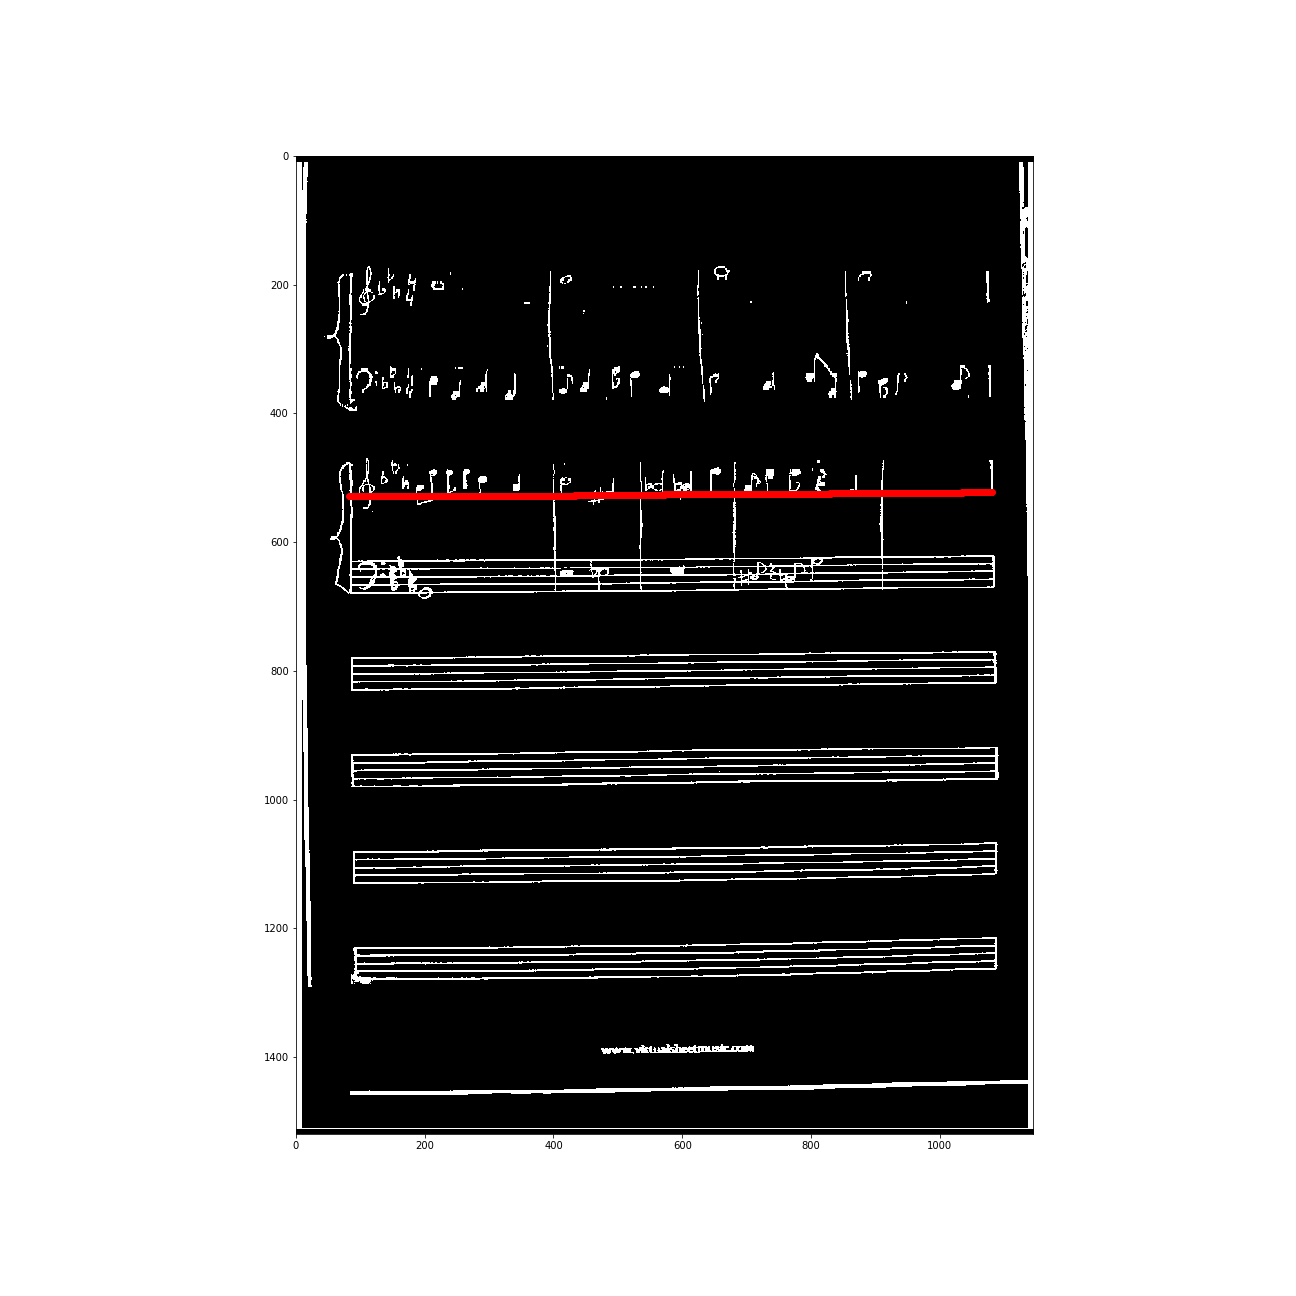
\includegraphics[width=\linewidth]{zdj/BFS15.png}
		\end{subfigure}
		\begin{subfigure}[b]{0.32\linewidth}
			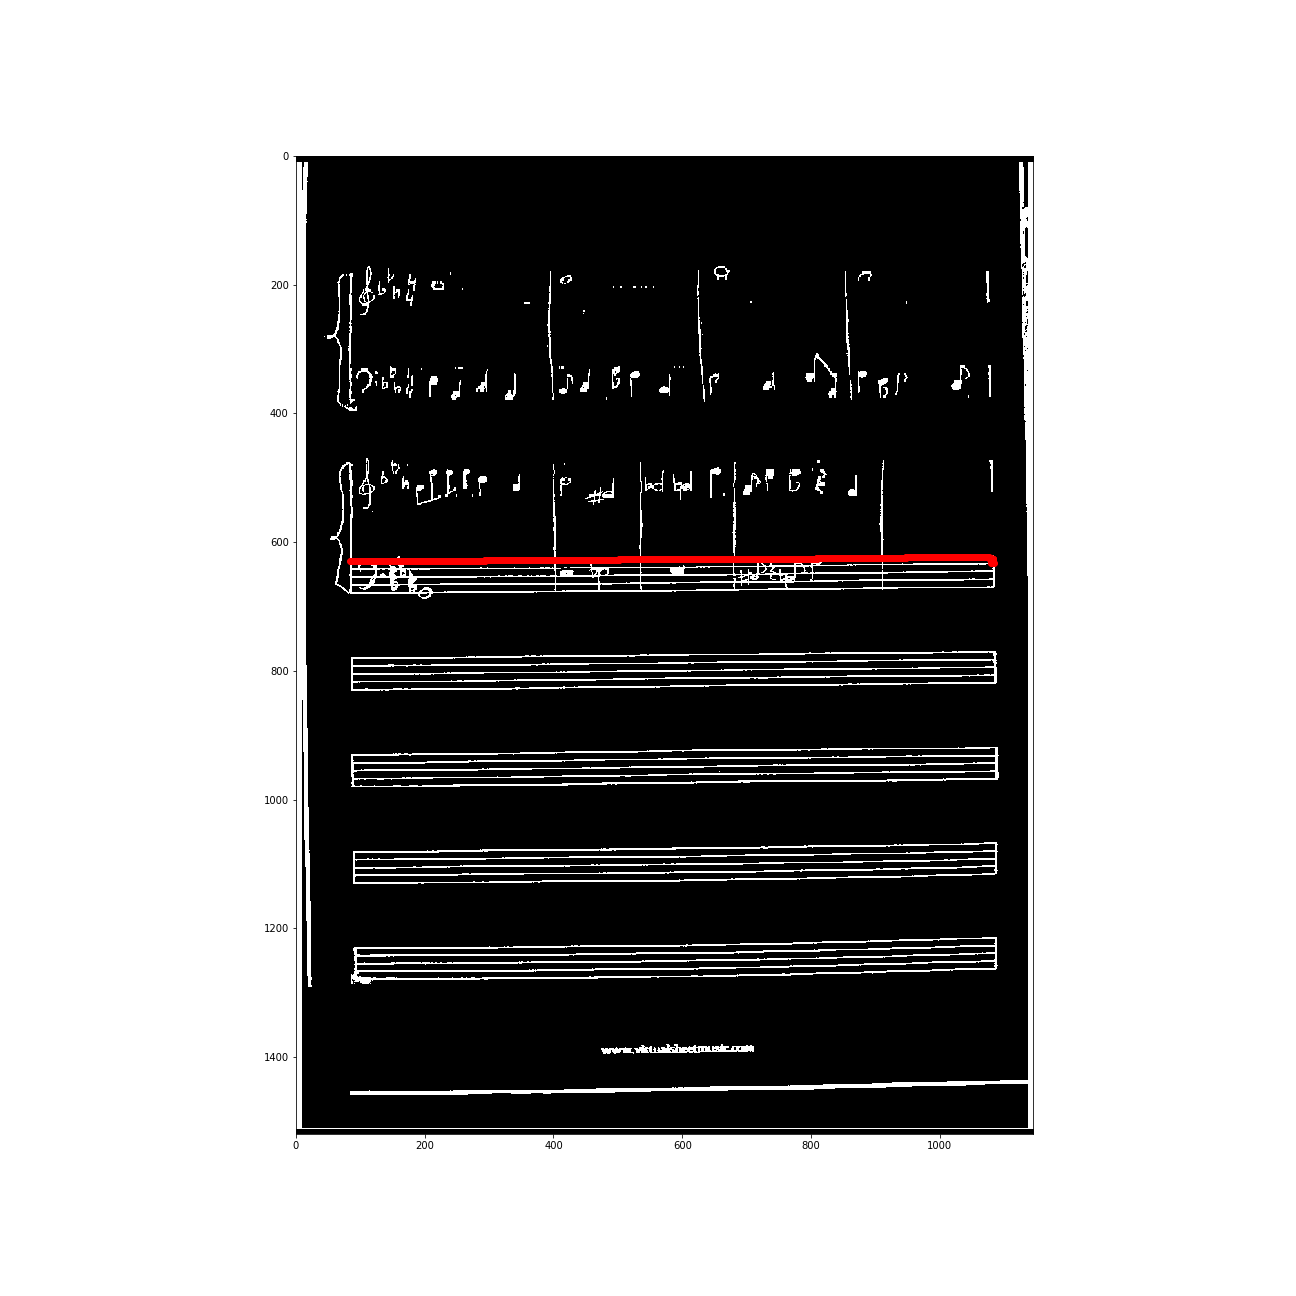
\includegraphics[width=\linewidth]{zdj/BFS16.png}
		\end{subfigure}
		\begin{subfigure}[b]{0.32\linewidth}
			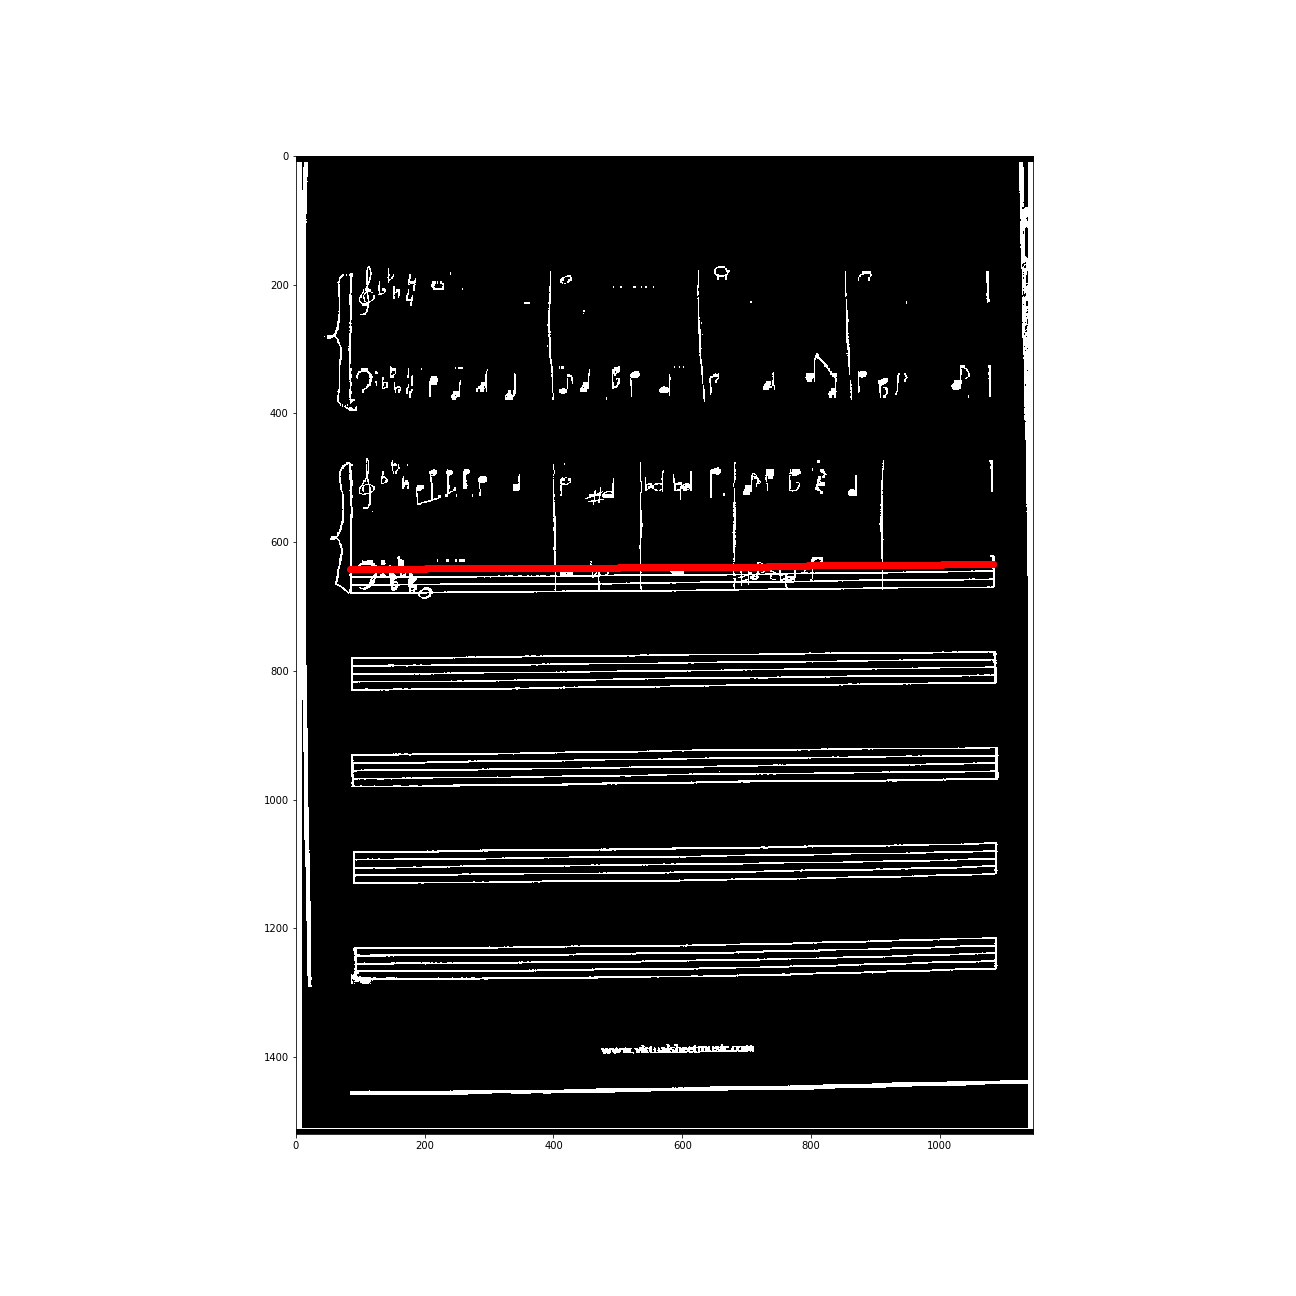
\includegraphics[width=\linewidth]{zdj/BFS17.png}
		\end{subfigure}
		\begin{subfigure}[b]{0.32\linewidth}
			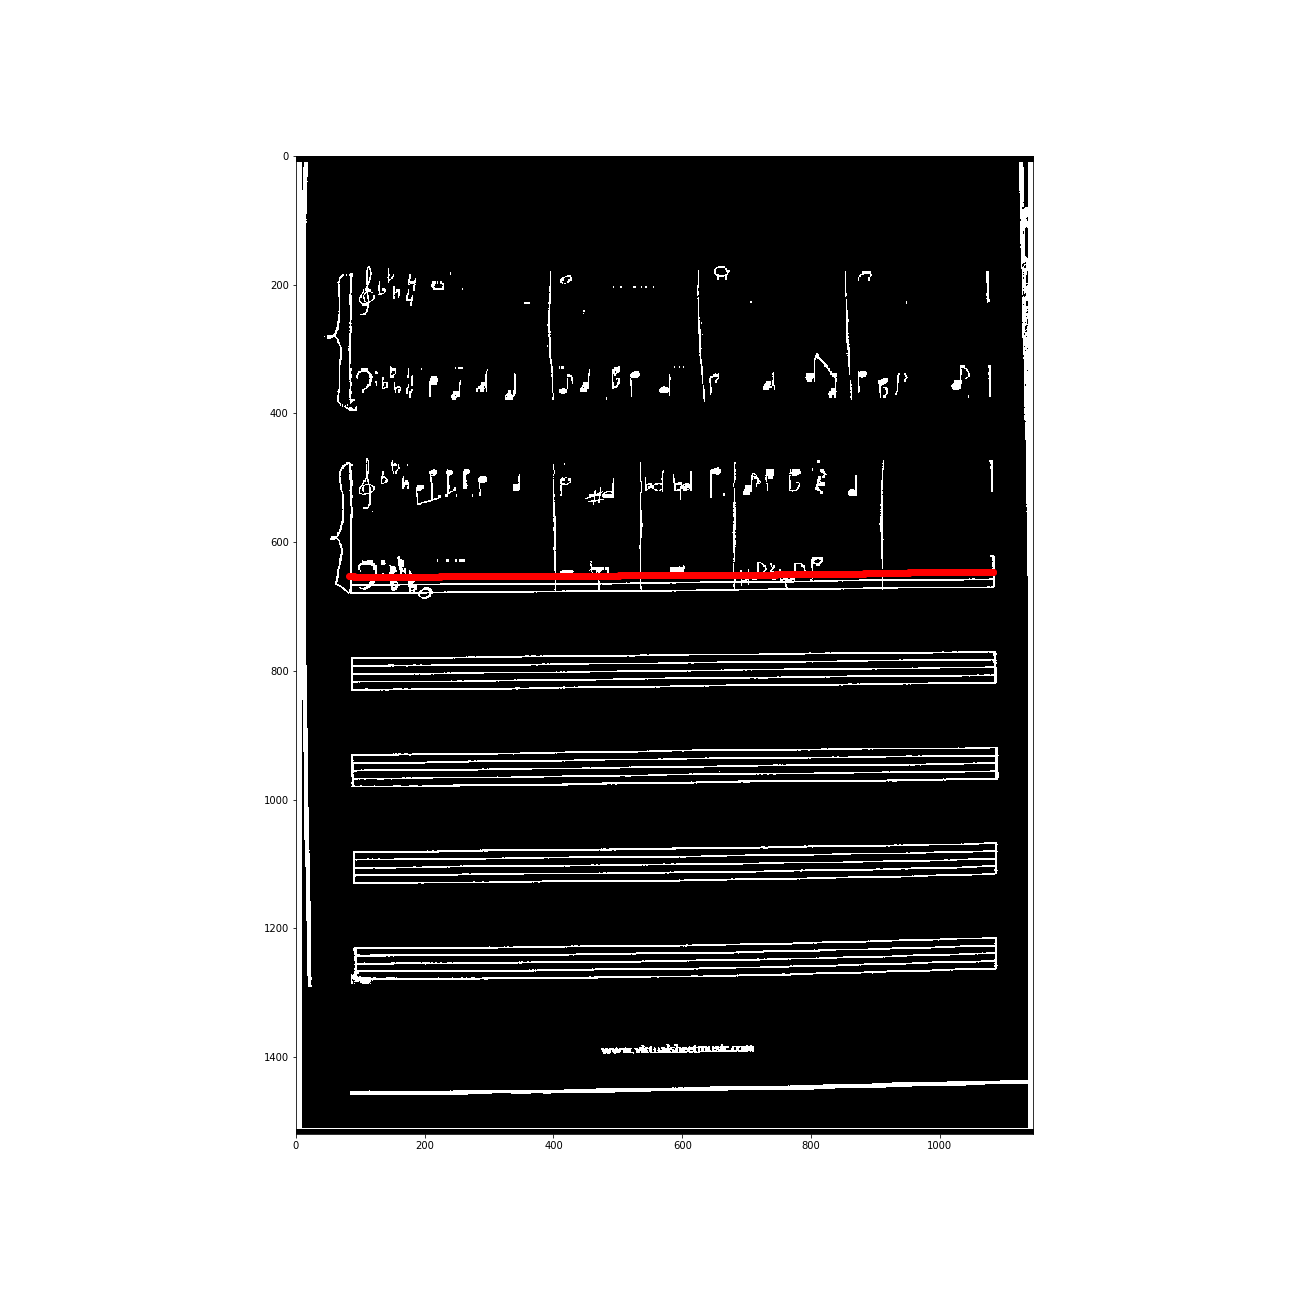
\includegraphics[width=\linewidth]{zdj/BFS18.png}
		\end{subfigure}
		\begin{subfigure}[b]{0.32\linewidth}
			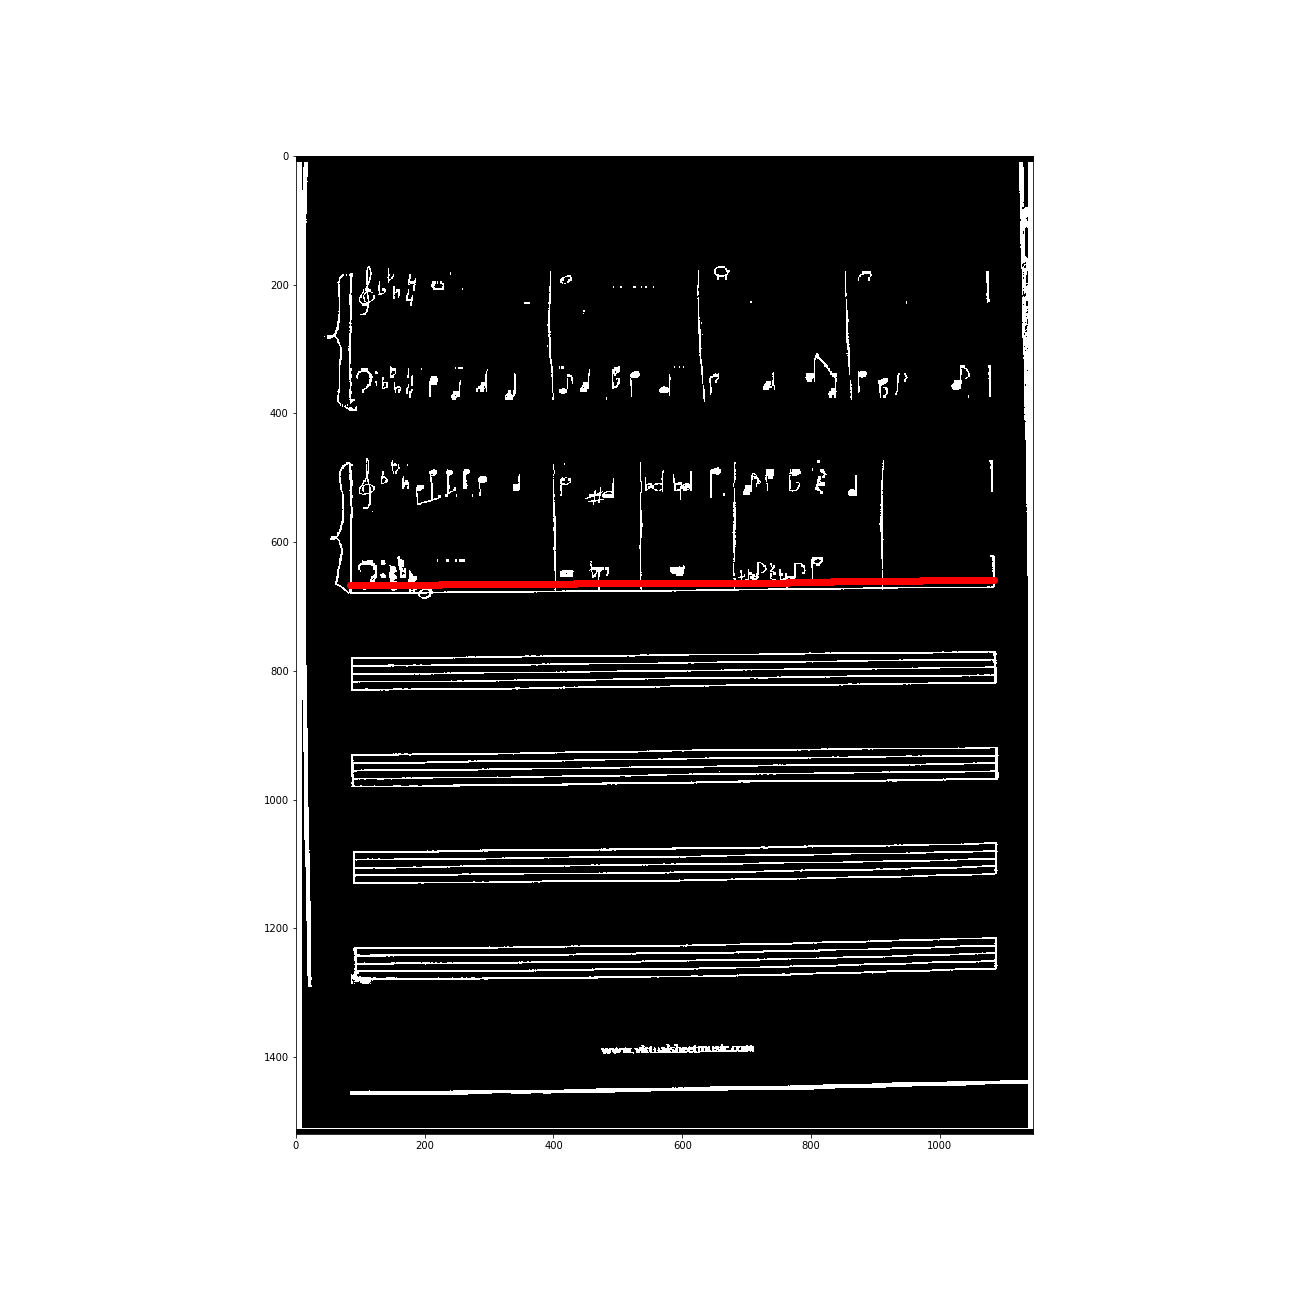
\includegraphics[width=\linewidth]{zdj/BFS19.png}
		\end{subfigure}
		\begin{subfigure}[b]{0.32\linewidth}
			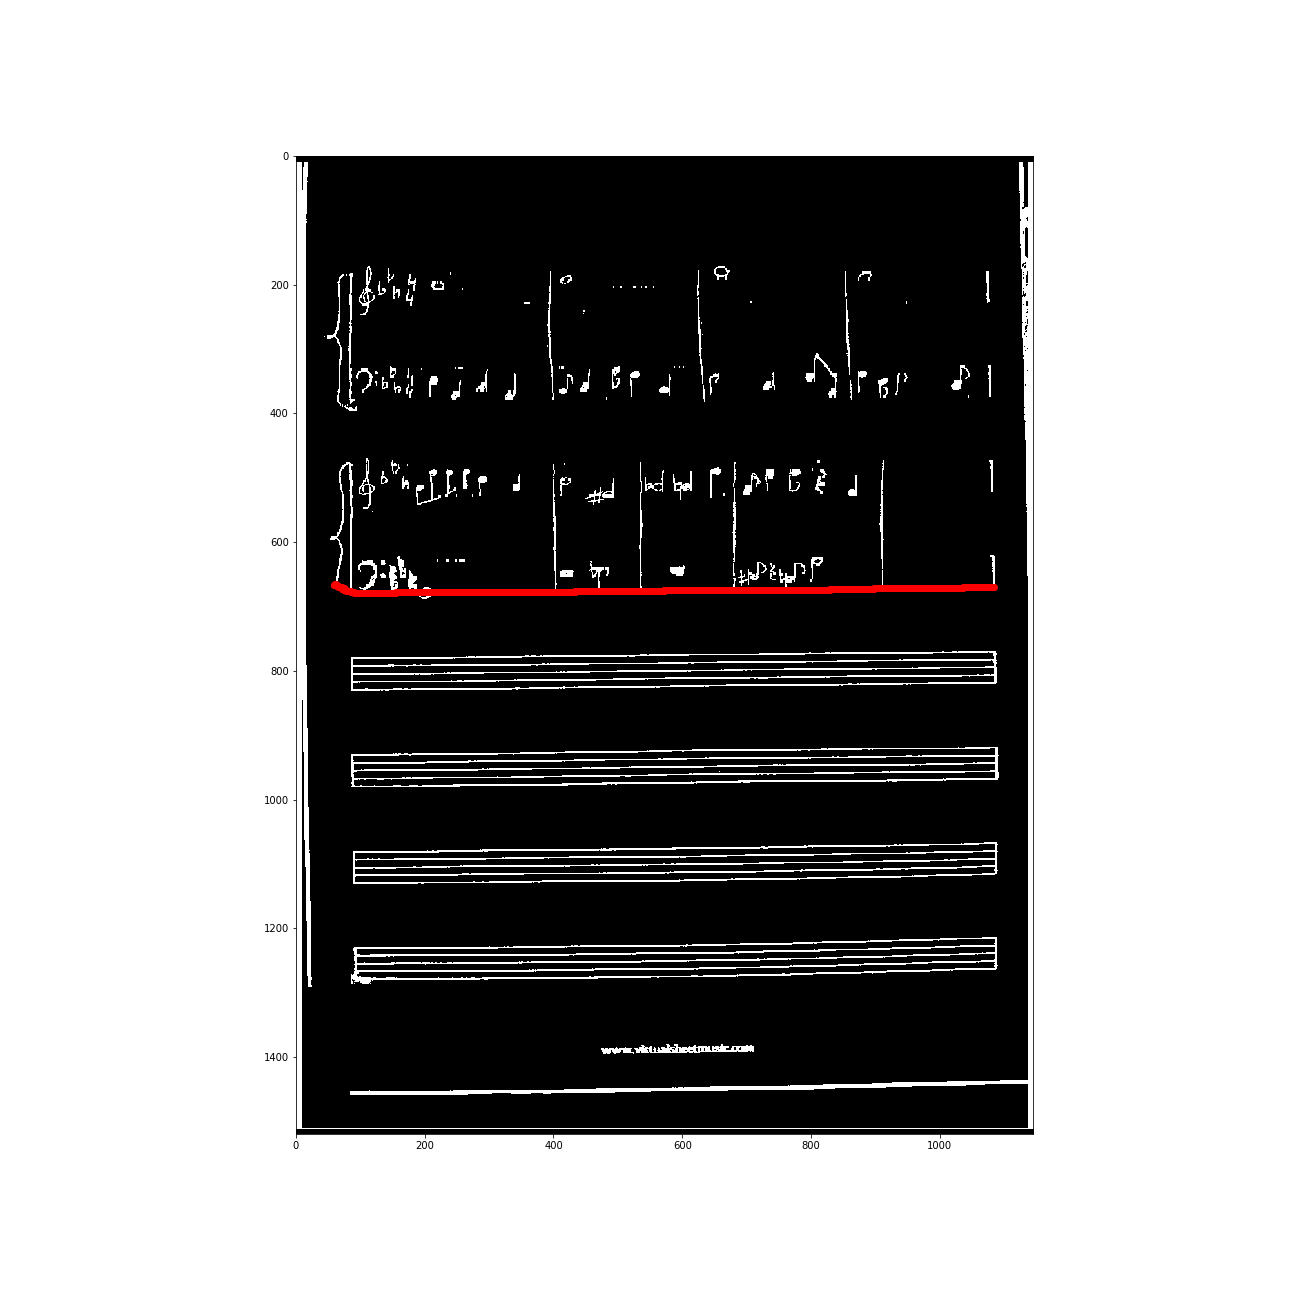
\includegraphics[width=\linewidth]{zdj/BFS20.png}
		\end{subfigure}
		\begin{subfigure}[b]{0.32\linewidth}
			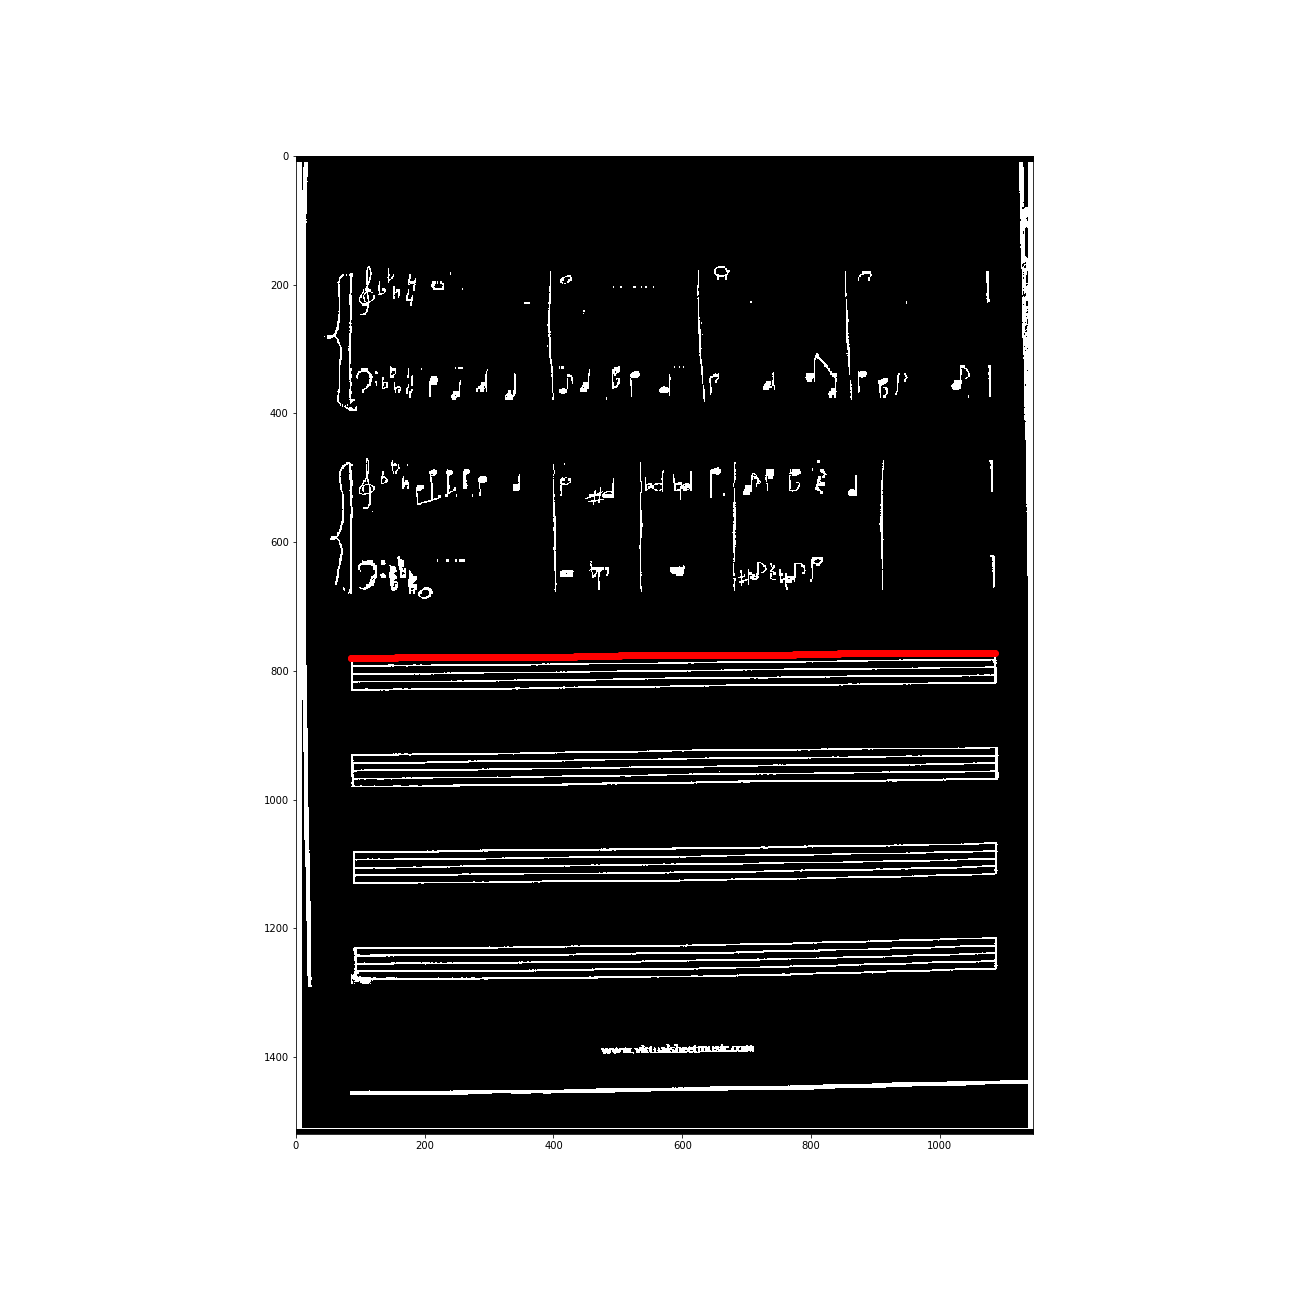
\includegraphics[width=\linewidth]{zdj/BFS21.png}
		\end{subfigure}
		\begin{subfigure}[b]{0.32\linewidth}
			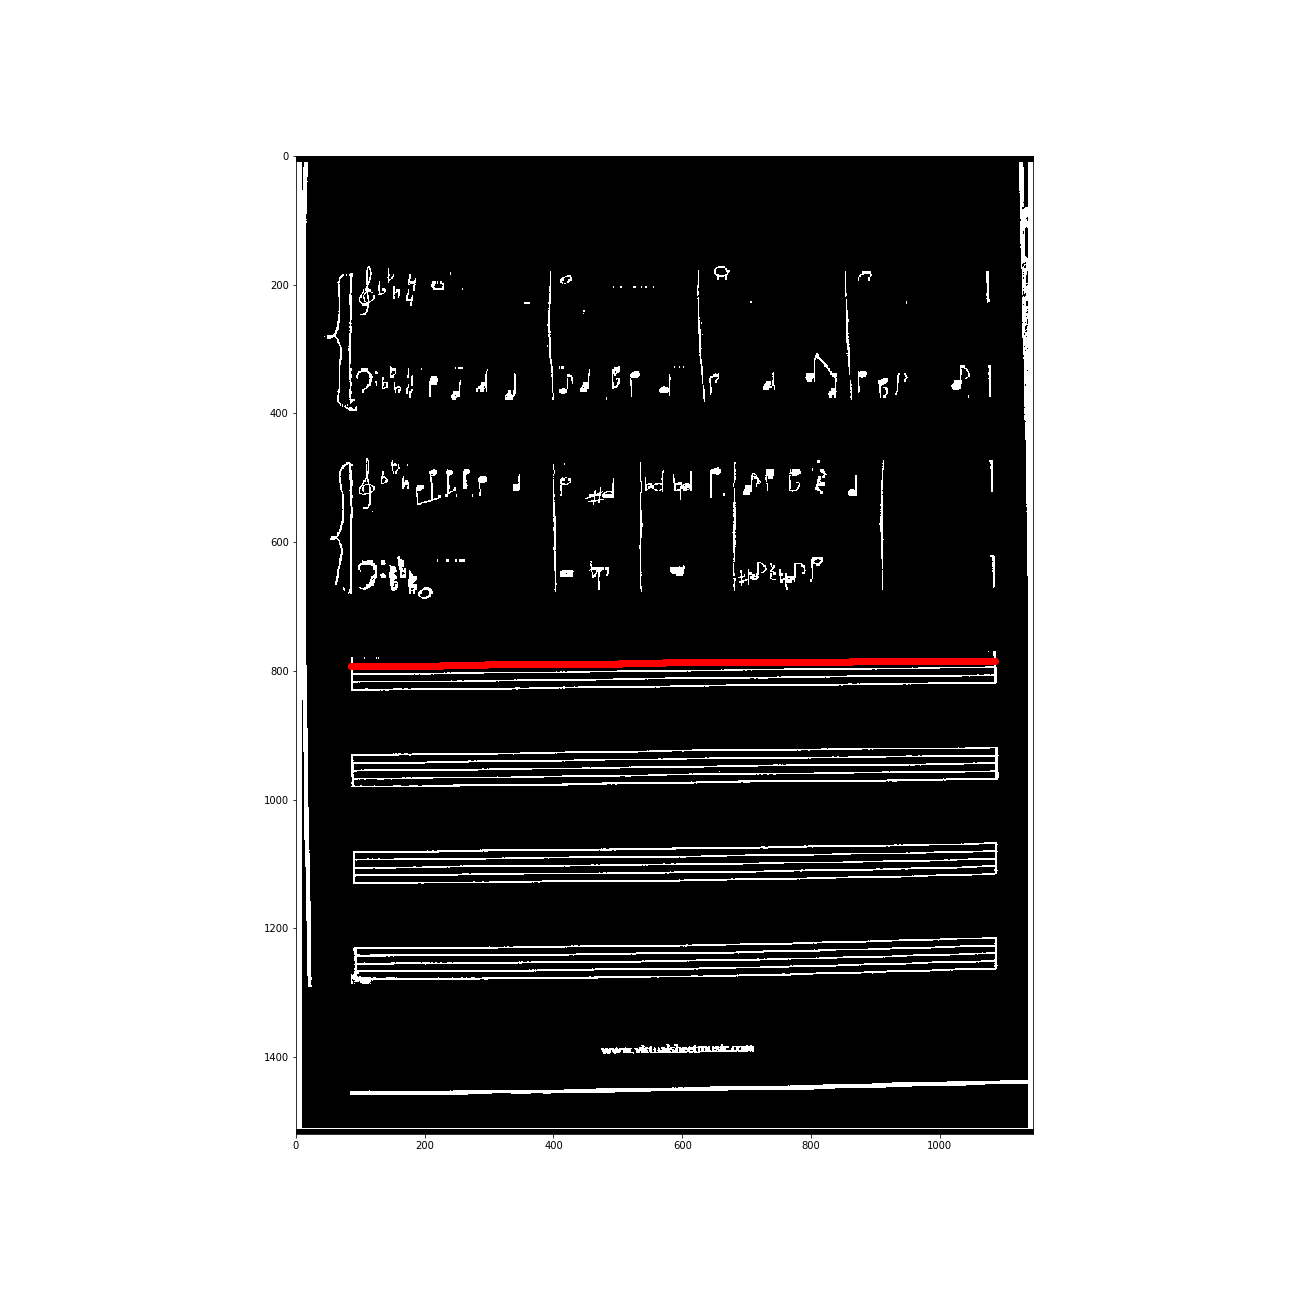
\includegraphics[width=\linewidth]{zdj/BFS22.png}
		\end{subfigure}
		\begin{subfigure}[b]{0.32\linewidth}
			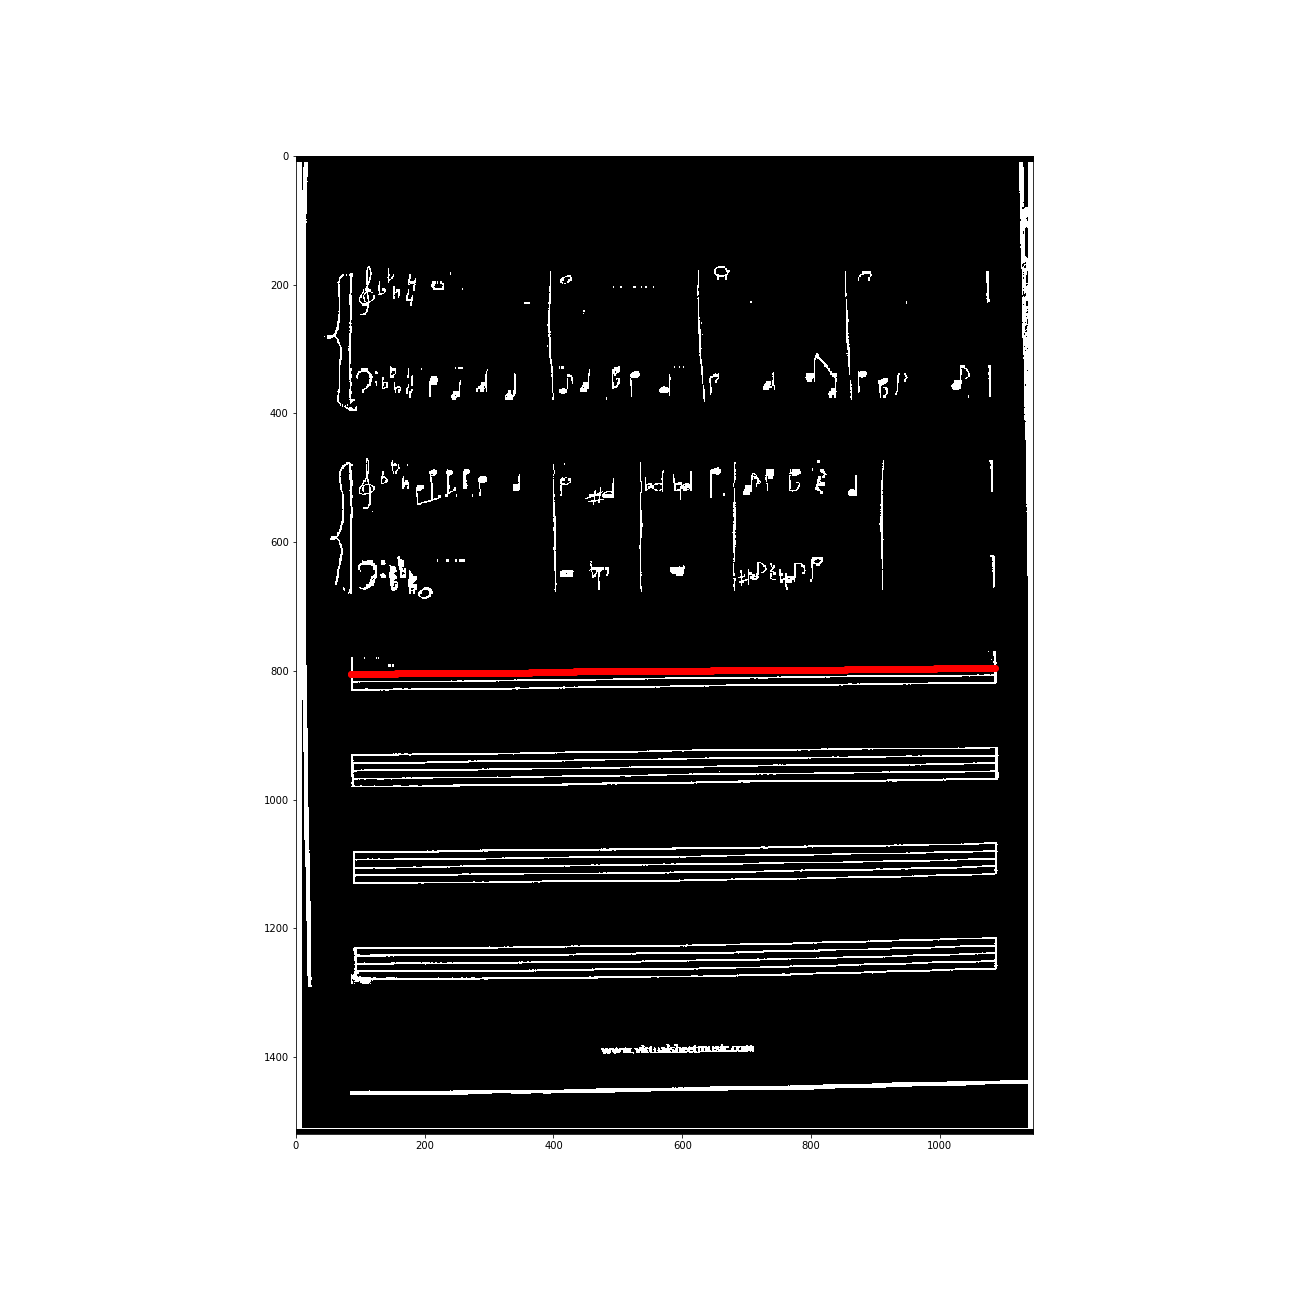
\includegraphics[width=\linewidth]{zdj/BFS23.png}
		\end{subfigure}
		\caption{Proces Detekcji i usuwania linii 2.}
		\label{fig:bfs1}
	\end{figure}

	\begin{figure}[h!]
		\centering
		\begin{subfigure}[b]{0.48\linewidth}
			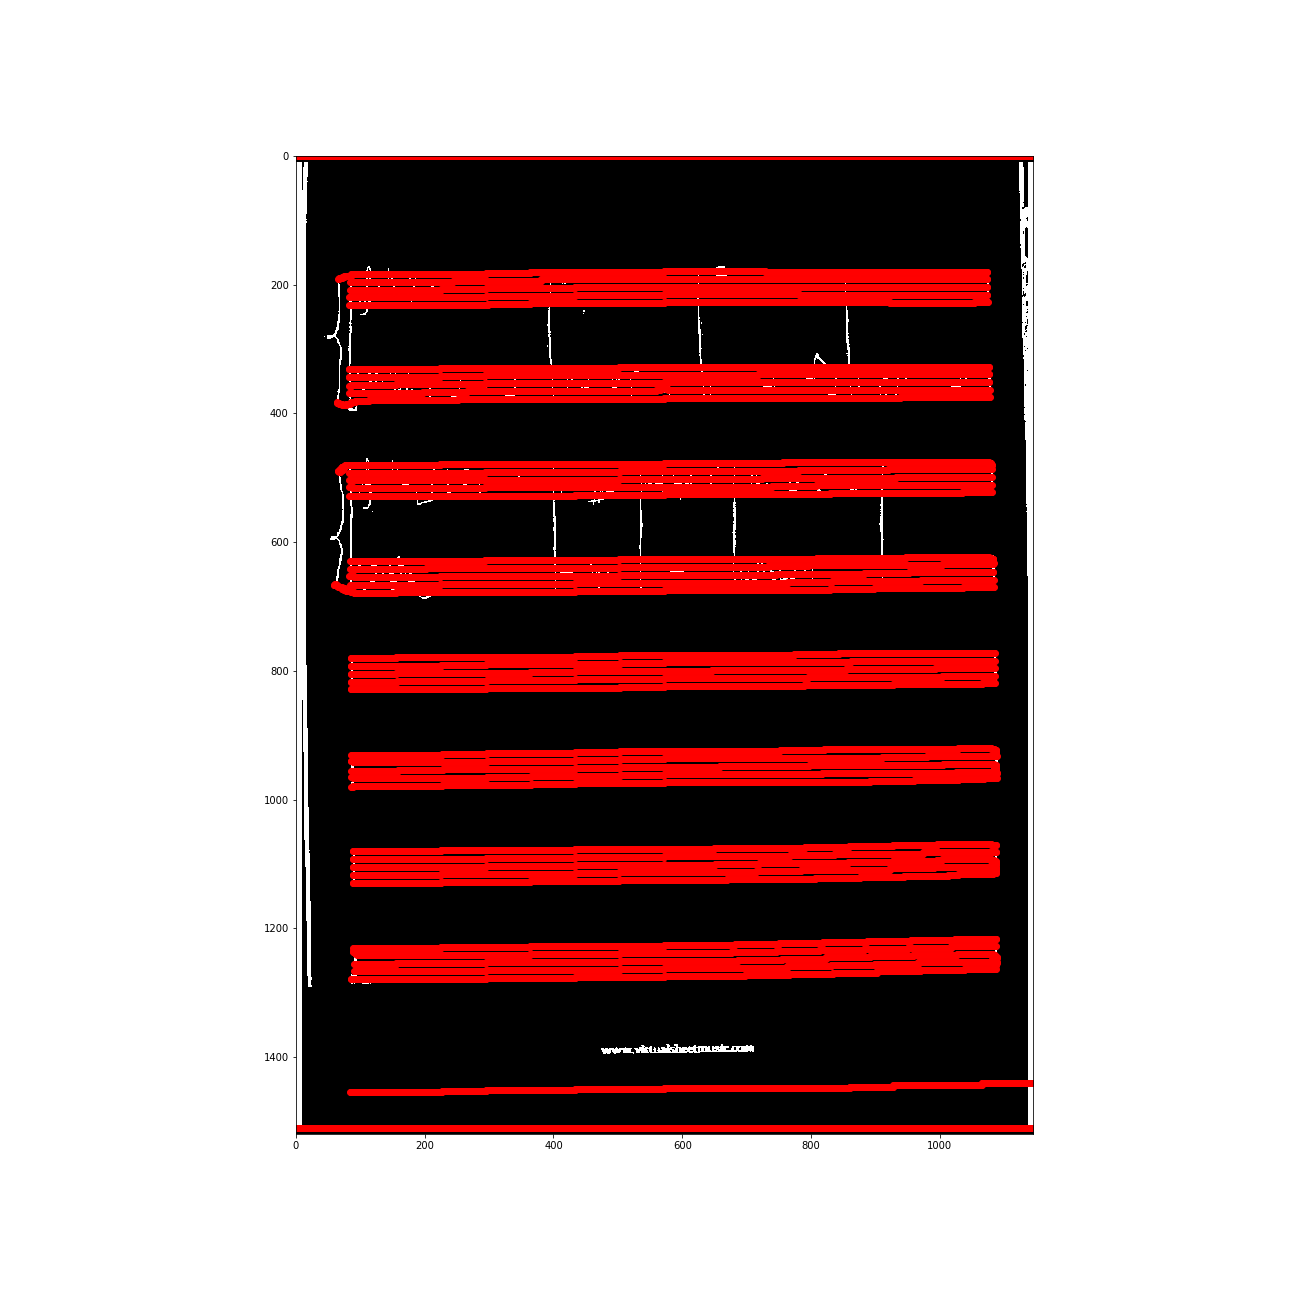
\includegraphics[width=\linewidth]{zdj/BFSFinale0.png}
			\caption{To, co ścięto}
		\end{subfigure}
		\begin{subfigure}[b]{0.48\linewidth}
			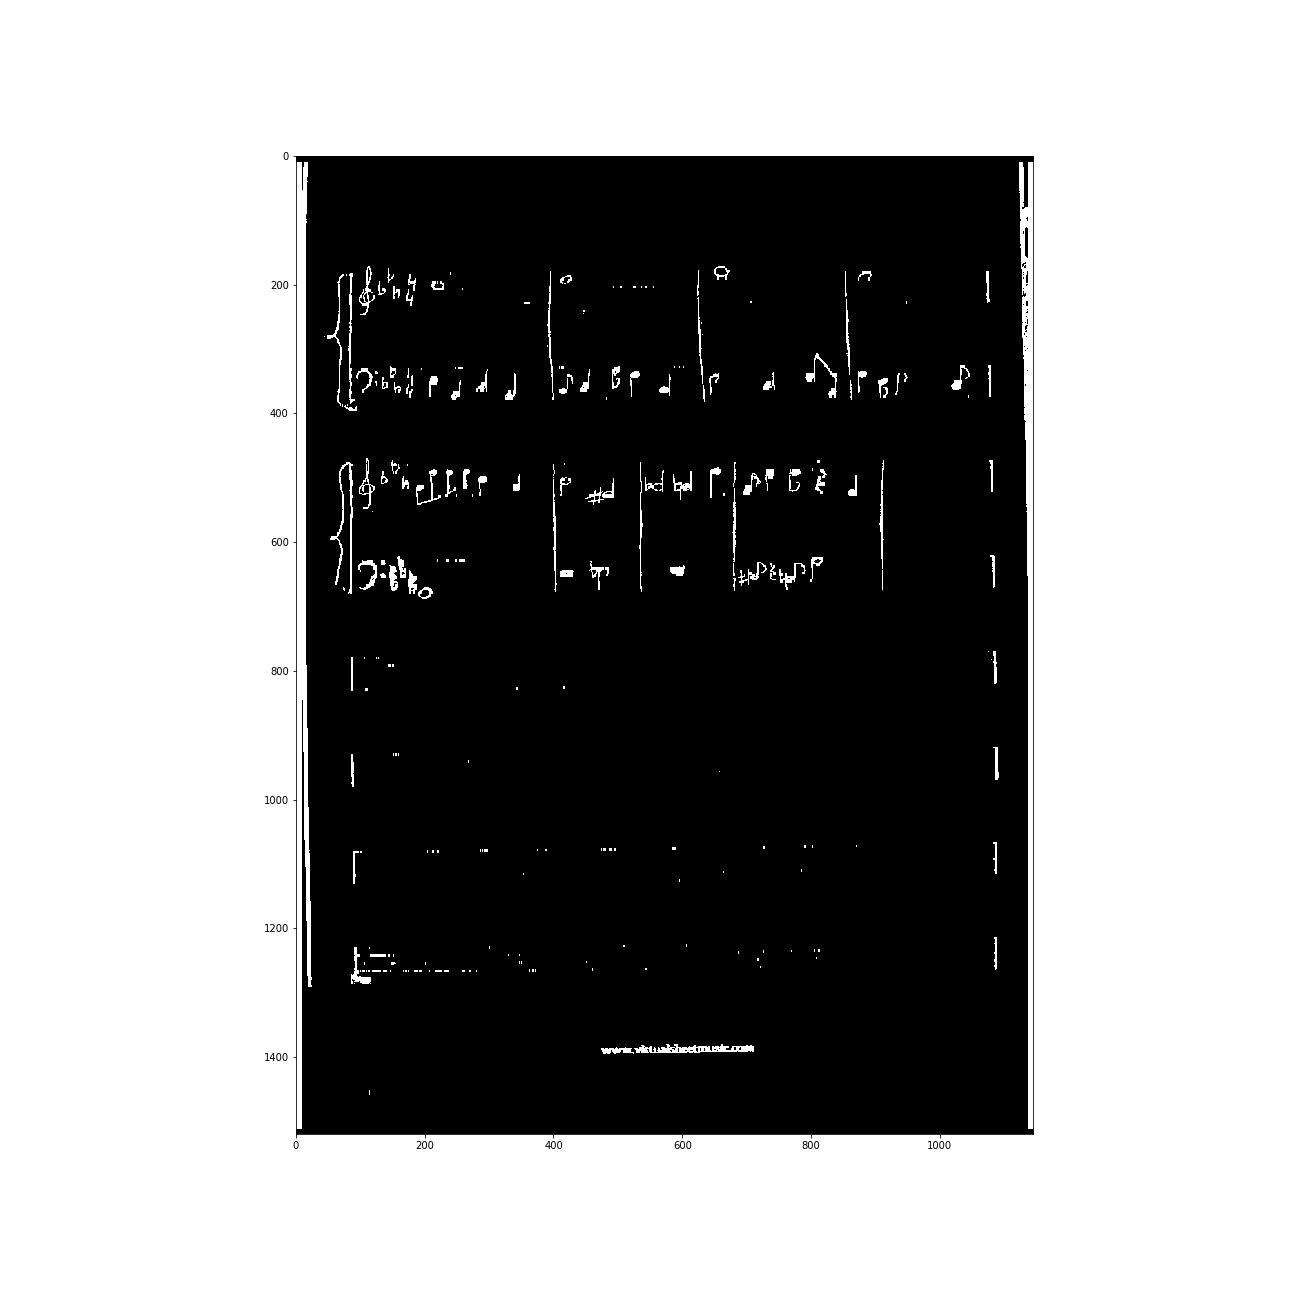
\includegraphics[width=\linewidth]{zdj/BFSFinale1.png}
			\caption{To, co zostało}
		\end{subfigure}
		\caption{Ostateczny efekt BFS-a.}
		\label{fig:bfsfinale}
	\end{figure}
	
	\begin{figure}[h!]
		\centering
		\begin{subfigure}[b]{0.48\linewidth}
			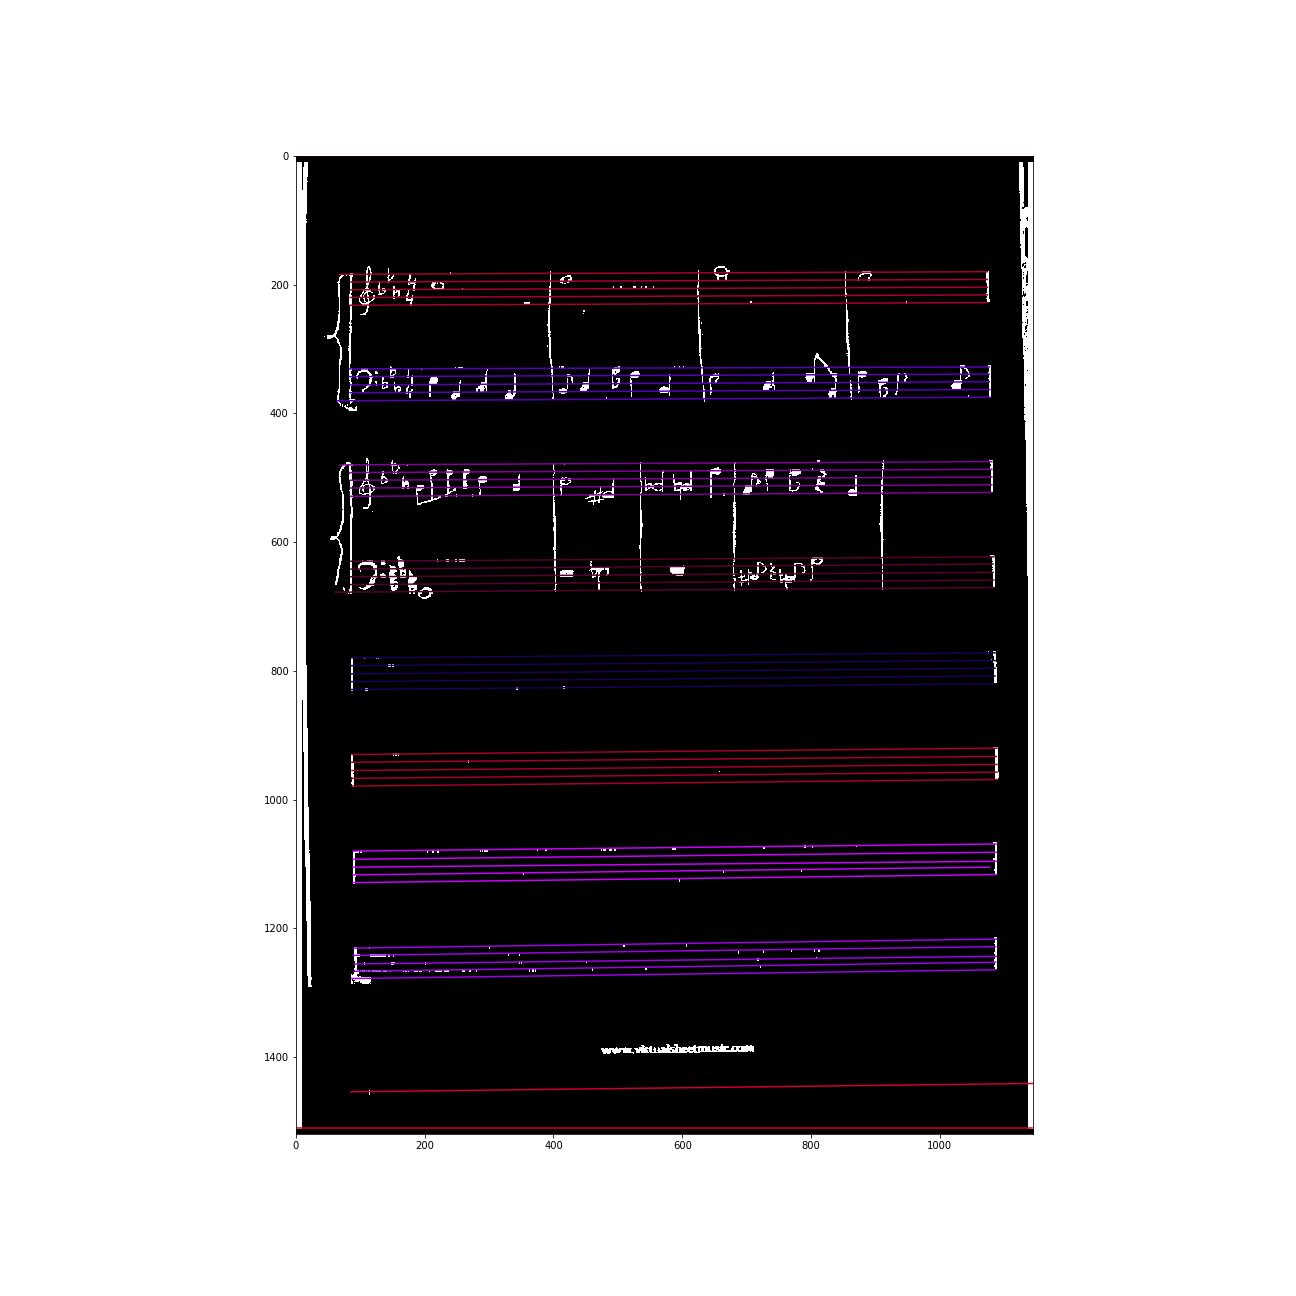
\includegraphics[width=\linewidth]{zdj/5l0.png}
			\caption{Wszystkie linie zgrupowane}
		\end{subfigure}
		\begin{subfigure}[b]{0.48\linewidth}
			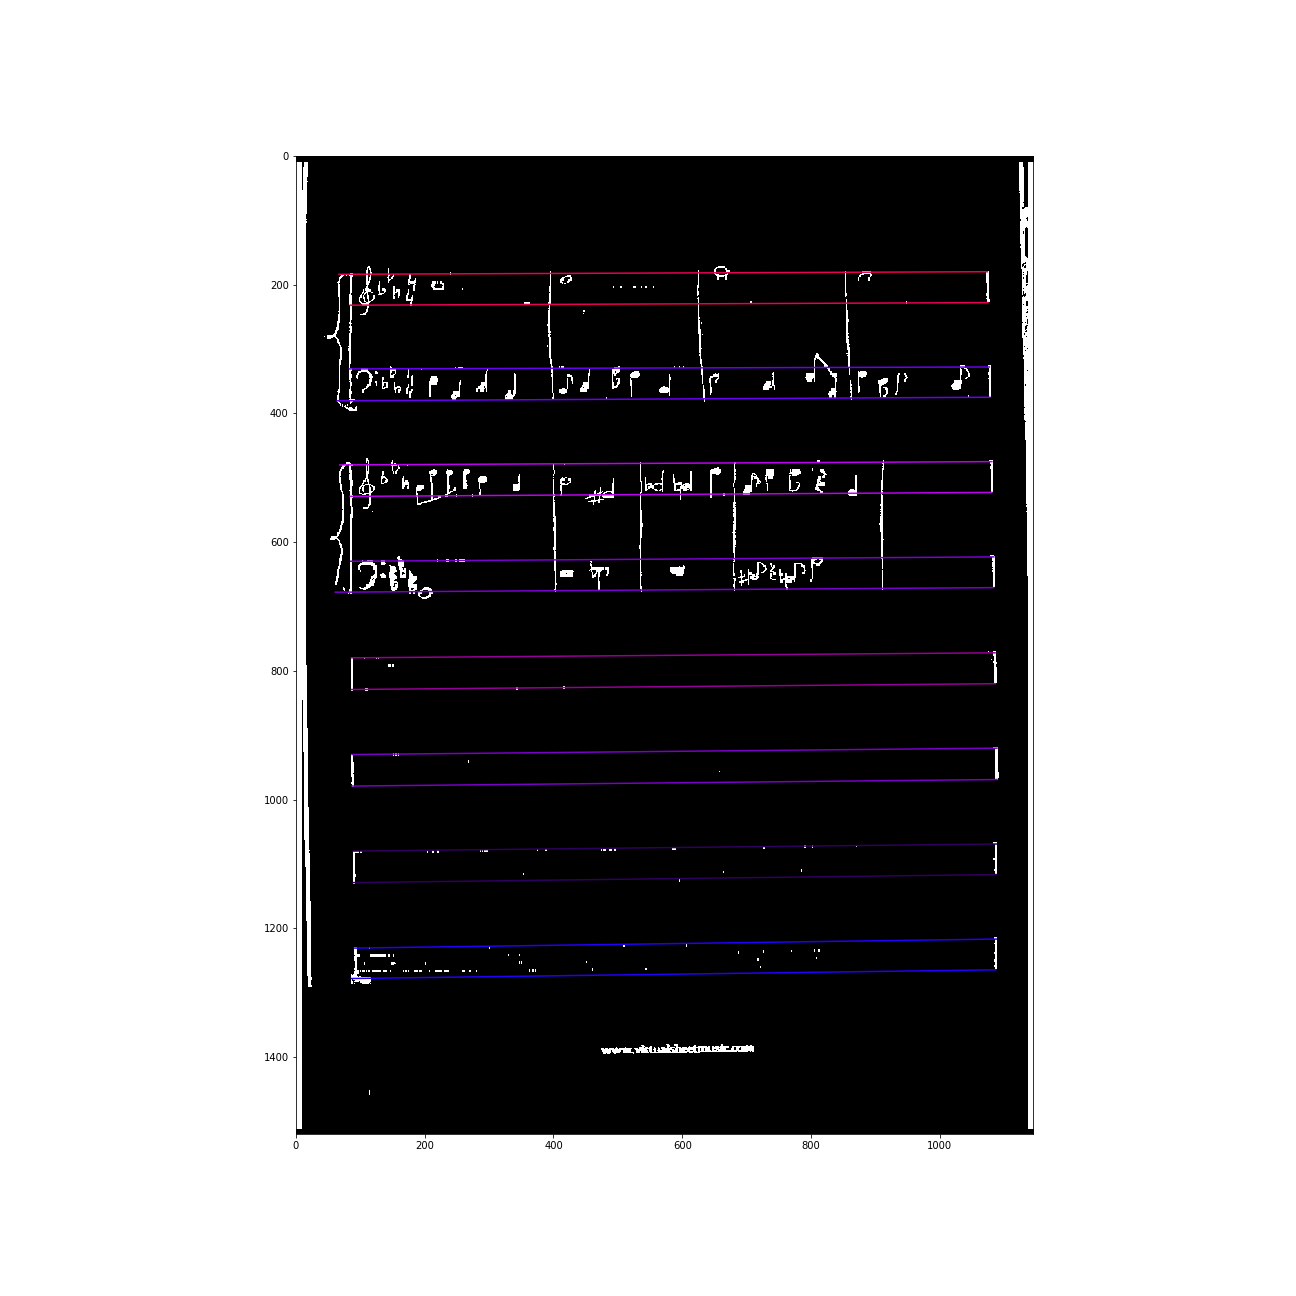
\includegraphics[width=\linewidth]{zdj/5l1.png}
			\caption{Linie po odsiewie}
		\end{subfigure}
		\caption{Poszukiwanie pięciolinii}
		\label{fig:5l}
	\end{figure}
%...



\end{document}

